
%\documentstyle[aps,prl,twocolumn,showpacs,amsmath,amssymb]{revtex4}

%\documentclass[twocolumn]{article}
\documentclass[a4paper]{article}
\usepackage{graphicx}
\usepackage{amsmath}
\usepackage{amssymb}
\usepackage{fullpage}


\def\D{{\cal D}}

\def\be{\begin{equation}}
\def\ee{\end{equation}}
\def\bea{\begin{eqnarray}}
\def\eea{\end{eqnarray}}
\def\bma{\begin{mathletters}}
\def\ema{\end{mathletters}}
\def\P{{\cal P}}
\def\0{\overline{0}}
\def\p{\overline{\pi}}
\def\q0{\underline{0}}
\def\qp{\underline{\pi}}
\def\H{{\cal H}}
\def\Z{{\cal Z}}
\def\S{{\cal S}}
\def\C{{\cal C}}

\def\sz{{\sigma_z}}
\def\sx{{\sigma_x}}
\def\sy{{\sigma_y}}

\def\E{{\cal E}}
\def\W{{\cal W}}
\def\L{{\cal L}}
\def\U{{ U}}
\def\R{{\cal R}}
\def\w{{\mbox w}}
\def\r{{\mbox r}}
\def\tr{\mbox{tr}}
\def\one{\leavevmode\hbox{\small1\normalsize\kern-.33em1}}
\def\compl{\begin{picture}(8,8)\put(0,0){C}\put(3,0.3){\line(0,1){7}}\end{picture}}


\def\bra#1{\langle#1|} \def\ket#1{|#1\rangle}
\def\braket#1#2{\langle#1|#2\rangle}
\def\bracket#1#2{\langle#1,#2\rangle}
\def\proj#1{\ket{#1}\!\bra{#1}}
\def\ve#1{\langle#1\rangle}





\begin{document}
\title{ Quantum Communications and Cryptography
 }

%%%%%%%%%%%% Abstract %%%%%%%%%%%%%%%%%%%%%%%%%%%

\maketitle

\begin{center}
Antonio Ac\'\i n
\end{center}


These are the notes for the course on Quantum Communications and Cryptography of the Master of Quantum Science and Engineering at the University of Barcelona. We first give a summary of the mathematical
techniques required in the quantum formalism: how to represent
quantum states, their evolution and measurement. This defines the
rules common to any quantum information application. Then, we
present the basic unit of quantum information, the so-called quantum bit or
qubit. Then, we move to quantum cryptography, with an emphasis on quantum key distribution protocols. Finally, we discuss the problem of
long-distance quantum communication.

\section{Basics of Quantum Mechanics}

The scope of this first section is to introduce the basic
postulates of Quantum Mechanics and its mathematical structure.
Most of the formalism presented here can be found in chapter 2 of
\cite{NC}.

Linear algebra is the study of vector spaces and of linear
operators acting on those spaces. Actually, all quantum machinery is
linear algebra on a complex Hilbert space explained through the
less standard Dirac's notation. In this notation,
\begin{itemize}
    \item $\ket{\psi}$ stands for a column vector, also known as a
    \emph{ket}.
    \item $\bra{\psi}$ stands for the vector dual to $\ket{\psi}$, also known as
    \emph{bra}.
    \item $\langle\phi\ket{\psi}$ is the standard scalar
    product between two vectors $\ket{\psi}$ and
    $\ket{\phi}$.
\end{itemize}
Example: given two vectors on a two-dimensional complex space,
denoted by $\compl^2$,
\begin{equation}
    \ket{\psi}=\begin{pmatrix}1 \\i \\\end{pmatrix} \quad
    \ket{\phi}=\begin{pmatrix}-3i \\-1 \\\end{pmatrix} ,
\end{equation}
one has
\begin{equation}
    \bra{\psi}=\begin{pmatrix}1 &-i \\\end{pmatrix} \quad
    \langle\phi\ket{\psi}=\begin{pmatrix}3i &-1 \\\end{pmatrix}
    \begin{pmatrix}1 \\i \\\end{pmatrix}=2i .
\end{equation}
The norm of a vector $\ket{\psi}$ is
$||\psi||=\sqrt{\langle\psi\ket{\psi}}$. In general, most of Quantum Information (QI)
applications deal with complex spaces of finite dimension $d$, denoted by
$\compl^d$.

{\sl Pure states:} The first postulate of Quantum Mechanics says
that there is a complex Hilbert space (vector space with an inner
product) associated to any physical system. The
description of this system is given by a normalized vector in this
space. On the other hand, any normalized vector in the space represents a possible state of the physical system. 
Therefore, all the information
about an isolated physical system can be specified by means of a vector
in a Hilbert space.
It follows from this postulate and the definition of a
vector space that if $\ket{\psi_1},\ket{\psi_2}\in\compl^d$ are
two possible states of a system, then any linear superposition of
these two vectors, $\ket{\psi}=\alpha\ket{\psi_1}+\beta\ket{\psi_2}$,
where $\alpha$ and $\beta$ are complex numbers and such that
$||\Psi||=1$, is a valid vector and, hence, also represents a valid state of the system.
This is also known as the \emph{superposition principle} and
$\ket{\psi}$ is often called a coherent superposition of
$\ket{\psi_1}$ and $\ket{\psi_2}$. 

{\sl Composite systems:} Consider now two physical systems, $A$ and
$B$, each described by the corresponding Hilbert space, $\H_A$ and
$\H_B$. The Hilbert space associated to the global system $AB$,
denoted by $\H$, consists of the tensor product of the two local
spaces, $\H=\H_A\otimes \H_B$. This is another postulate of Quantum
Mechanics. 

{\sl Entanglement:} The consequences of these two initial postulates
 are huge.
Indeed, consider two possible states of the global system,
$\H_A\otimes\H_B$, $\ket{\psi_A}\otimes\ket{\psi_B}$, or more
briefly $\ket{\psi_A\psi_B}$, and $\ket{\phi_A\phi_B}$. Then,
$\ket{\Psi}=\alpha\ket{\psi_A\psi_B}+\beta\ket{\phi_A\phi_B}$ also
gives a possible state of the composite system $AB$. However, this
state in general cannot be written as the tensor product of two
vectors on each local space, $\ket{\Psi}\neq
\ket{\varphi_A\varphi_B}$. It is said that $\ket{\Psi}$ is
\emph{entangled}. Entanglement then appears as a consequence of
the tensor product and vector space structure of Quantum
Mechanics. 

{\sl Unitary evolution:} The evolution of an isolated physical
system, whose initial state is given by $\ket{\psi}$, is described
by the application of a unitary operation, $U$. Thus, the evolved
state of the system is $\ket{\phi}=U\ket{\psi}$. Recall that this
is another postulate of Quantum Mechanics. A unitary operation on
a Hilbert space of dimension $d$ is simply a $d\times d$ complex matrix
satisfying $U U^\dagger=\one$.

{\sl Mixed states:} Consider the previous description of
entanglement: a state is entangled when it cannot be written in a
product form. That is, although the global state of the system can
be described by a vector in $\H_A\otimes\H_B$, it is impossible to
associate to each local system a vector in $\H_A$ and $\H_B$. This
is indeed related to the fact that system $A$ is correlated to
$B$, it is not isolated. Is there a mathematical way of describing
non-isolated systems?

Alternatively, consider the case in which the preparation of a
system is imperfect, that is, the system can be in state
$\ket{\psi_1}$ with probability $p_1$, $\ket{\psi_2}$ with
probability $p_2$ and so on. What's the mathematical description
of the state of the system? Notice that in both cases there is a
lack of knowledge about the state of the system. This is evident
in the second scenario, since the preparation is noisy. But the
same also happens in the first case: when trying to describe the
local state of a non-isolated system, all the correlations with
other systems, the environment, are ignored. Since the information
on the state of the system is not complete, the state cannot be
pure. In order to take into account this lack of information, 
the concept of mixed states is introduced.

The mathematical description of a system that can be in state
$\ket{\psi_i}\in\H$ with probability $p_i$, where $i=1,\ldots,N$
and $N$ is arbitrary, is no longer given by a vector in this Hilbert space, 
but by an operator acting on it with the form
\begin{equation}\label{mixst}
    \rho=\sum_{i=1}^N p_i\proj{\psi_i} .
\end{equation}
Note that $\tr(\rho)=\sum p_i\,\tr(\proj{\psi_i})=\sum_i p_i\,
\langle\psi_i\ket{\psi_i}=\sum_i p_i=1$. If the state is pure,
$\ket{\psi}$, there is only one non-vanishing probability, $p_1=1$,
and $\rho=\proj{\psi}$. Actually, a state $\rho$ is pure if, and
only if, $\tr\rho^2=1$.

{\sl Noisy evolution:} Having introduced the mixed-state
formalism, one can specify how an open quantum system evolves, or
how to describe a noisy evolution. In this case, a quantum system
in a pure state may loose its purity and become mixed. The general
formalism is given by trace preserving completely positive maps. Indeed,
any evolution of an initial state, possibly mixed, $\rho_i$, into
a state $\rho_f$, can be represented as
\begin{equation}\label{krausop}
    \rho_f=\sum_k A_k \rho_i A^\dagger_k ,
\end{equation}
where $A_k$ are operators such that $\sum A_kA^\dagger_k=\one$. Note that $\rho_f$ is
positive and has trace one.

{\sl Measurements:} The last process to consider is a
measurement. Any measurement of $m$ outcomes on a system whose
associated Hilbert space has dimension $d$ can be represented by the so-called
Positive-Operator Valued Measure (POVM), defined by
$r$  positive operators $\{M_i\geq 0\}$, where
$i=1,\ldots,r$, such that $\sum_i M_i=\one$. Denote by $\rho$ the
state to be measured. Then, outcome $i$ is obtained with
probability $p\,(i|\rho)=\tr(\rho M_i)$, positive because $M_i$ are positive, and such that $\sum
p\,(i|\rho)=\sum_i \tr(\rho M_i)=\tr(\rho \sum_iM_i)=\tr(\rho)=1$. 

{\sl General evolution:} Collecting all the previous processes, a
general evolution, consisting of a sequence of measurements and
possibly noisy evolutions can always be specified through a set of
operators $A^i_k$ describing a map transforming any state $\rho$
into
\begin{equation}\label{genev}
    \rho_i=\frac{\sum_k A^i_k \rho A^{i\dagger_k}}
    {\tr(\sum_k A^i_k \rho A^{i\dagger}_k)} \quad \text{with probability}\quad p_i=\tr(\sum_k A^i_k \rho A^{i\dagger}_k).
\end{equation}


Standard von Neumann measurements are covered by
the previous formalism. A von Neumann, or projective measurement
in a $d$-dimensional system has $d$ possible outcomes and the
corresponding operators are the projectors onto a basis in this
space. More precisely: consider a basis in $\compl^d$, defined by 
$d$ orthonormal vectors ${\ket{i}}$ such that $\langle
i\ket{j}=\delta_{ij}$. A measurement in this basis is represented
by the projectors $A_i=\proj{i}$. Note that if the initial state
is $\rho$, the probability of obtaining outcome $i$, see Eq.~\eqref{genev}, is
\begin{equation}\label{vnpr}
    p_i=\tr(\proj i\rho\proj i)=\bra i\rho\ket i ,
\end{equation}
while the state is mapped into
\begin{equation}\label{vnev}
    \rho_i=\frac{\proj i\rho \proj i}
    {\tr(\proj i \rho \proj i)}=\proj i .
\end{equation}
For the pure-state case, $\rho=\proj\psi$, these expressions read
\begin{equation}\label{vnprpst}
    p_i=\tr(\proj i\proj\psi\proj i)=|\langle i\ket{\psi}|^2 ,
\end{equation}
and
\begin{equation}\label{vnev}
    \ket{\psi_i}=\ket i ,
\end{equation}
that is, the initial state $\ket{\psi}$ collapses into $\ket i$
with probability given by the square of the overlap, $|\langle
i\ket{\psi}|^2$. The previous formulae also imply that there is no
measurement (physical process) distinguishing $\ket{\psi}$ from
$e^{i\gamma}\ket{\psi}$. Thus, the state of a physical system is
actually described by a vector in a Hilbert space, up to an
irrelevant global phase.

\section{Basics elements of Quantum Information Theory}

The previous section summarizes the quantum formalism and presents
the main tools that will be needed in what follows. In this section,
we introduce some of the most basic concepts in Quantum Information Theory (QIT): the quantum bit and quantum
gates (or operations). Once all these concepts have been introduced,
we will illustrate through the no-cloning theorem and Bell's theorem how QIT can drastically depart from its classical counterpart.


\subsection{The quantum bit}

The first step is to introduce the basic unit of QI,
the quantum bit or qubit.
Consider the encoding of a classical bit into a quantum particle.
The way of doing this is by means of a two-dimensional system: bit
value 0 is encoded into a state $\ket{\psi_0}$, or simply
$\ket{0}$, and 1 into $\ket{1}$. Since these two options have to
define a classical bit, the states have to be orthogonal and give
a basis in $\compl^2$. Thus, a measurement in this basis
distinguishes in a deterministic way between the two
possibilities, as it happens for a classical bit. For instance,
\begin{equation}\label{2basis}
    \ket 0=\begin{pmatrix}1\\0\\\end{pmatrix}\quad\quad
    \ket 1=\begin{pmatrix}0\\1\\\end{pmatrix} .
\end{equation}
A two-dimensional quantum particle can encode a classical bit and
then defines a quantum bit. Note however that, because of the
superposition principle, any coherent combination of $\ket 0$ and
$\ket 1$ is also allowed, something that is classically
impossible. Therefore a quantum bit can be in any state,
\begin{equation}\label{qubit}
    \ket{\psi}=\alpha\ket 0+\beta\ket 1 ,
\end{equation}
where $\alpha$ and $\beta$ are complex numbers such that
$|\alpha|^2+|\beta|^2=1$.

It is possible to pictorially represent the state of a qubit, or
two-dimensional quantum particle, by means of the Poincar\'e
or Bloch sphere (see Fig. \ref{bloch}). Indeed, using
the fact that the global phase of any pure state is irrelevant,
$\alpha$ can always be taken real. Then, any quantum bit can be
specified by a complex number $\beta$, since $\alpha$ is fixed
because of normalization. That is, any state has the form
\begin{equation}
\label{blochv}
    \ket\psi=\begin{pmatrix}\cos\left(\frac{\theta}{2}\right)
    \\\sin\left(\frac{\theta}{2}\right)e^{i\varphi}\\\end{pmatrix}
    .
\end{equation}
Two angles $\theta$ and $\varphi$ suffice to specify any pure
state in $\compl^2$, as any point on the surface of a unit sphere.
It is important to mention here that given $\ket{\psi}$, the
orthogonal vector, $\ket{\psi_\perp}$, reads
\begin{equation}
\label{blochvorth}
    \ket{\psi_\perp}=\begin{pmatrix}\sin\left(\frac{\theta}{2}\right)
    \\-\cos\left(\frac{\theta}{2}\right)e^{i\varphi}\\\end{pmatrix}
    ,
\end{equation}
so orthogonal vectors in $\compl^2$ define antiparallel vectors on
the Bloch sphere.

Pauli matrices are going to play a significant role
in all what follows. Their expression is
\begin{equation}\label{pauli}
    \sigma_x=\begin{pmatrix}0&1\\1&0\\\end{pmatrix}\quad
    \sigma_y=\begin{pmatrix}0&-i\\i&0\\\end{pmatrix}\quad
    \sigma_z=\begin{pmatrix}1&0\\0&-1\\\end{pmatrix} .
\end{equation}
Note that in our definition of the qubit, $\ket 0$ and $\ket 1$
are the eigenvectors of $\sigma_z$ with eigenvalues $\pm 1$, since
$\sigma_z\ket i=(-1)^i\ket i$. This is why $\sigma_z$ is often
called a phase flip. Note that putting $\theta=0$ (and
$\varphi=\pi$) in (\ref{blochv}) and (\ref{blochvorth}), that is, Bloch
vectors pointing in the $\pm z$ direction, one obtains $\ket 0$
and $\ket 1$, the eigenvectors of $\sigma_z$. The effect of
$\sigma_x$ in our qubit basis is $\sigma_x\ket i=\ket{1-i}$, i.e.
it gives a bit flip. In a similar way as above, substituting
$(\theta,\varphi)=(\pi/2,0)$ and $(\theta,\varphi)=(\pi/2,\pi/2)$
in (\ref{blochv}) and (\ref{blochvorth}) gives the two eigenvectors of
$\sigma_x$ and $\sigma_y$, often denoted by $\ket{\pm x}$ and $\ket{\pm y}$.

\begin{figure}
\begin{center}
  % Requires \usepackage{graphicx}
  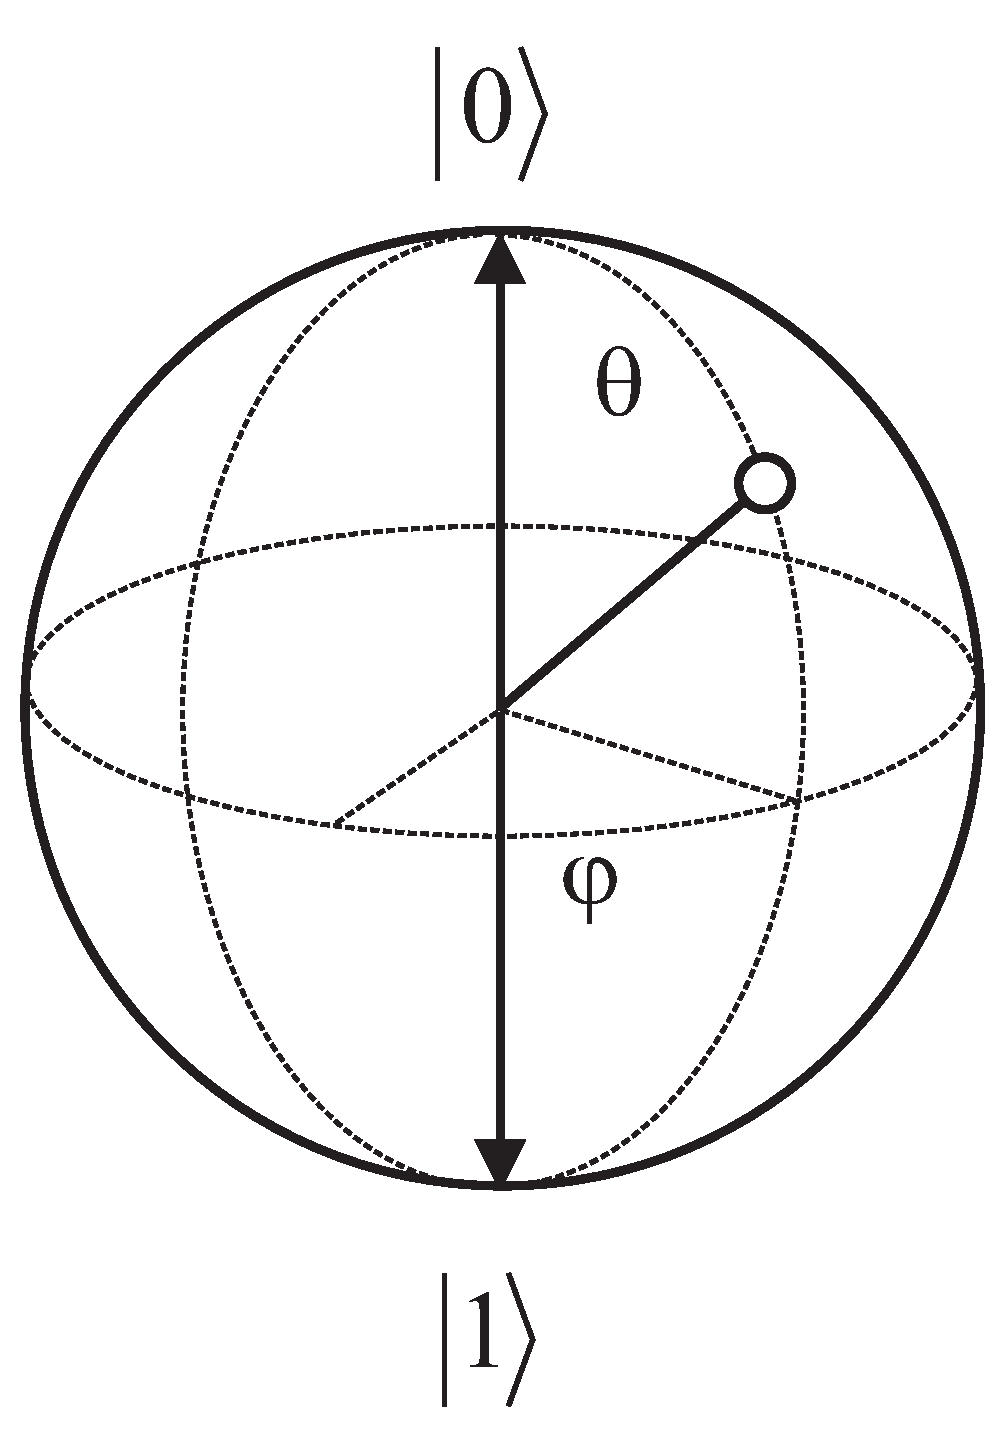
\includegraphics[width=5cm]{qubit}\\
  \caption{\textbf{Bloch sphere:} Any pure quantum bit can be represented
  by a point in the surface of the Bloch sphere. The corresponding
  unit vector, $\hat n=(\sin\theta\cos\varphi,\sin\theta\sin\varphi,
  \cos\theta)$, is known as Bloch vector. Mixed states
  are inside the sphere.}\label{bloch}
\end{center}
\end{figure}


\subsection{Quantum gates}


Although these notes focus on quantum communication and cryptography, let us briefly
review here, for the sake of completeness, the basic logical operations
acting on a qubit. Recall that any classical computation consists of a
sequence of logical gates on a string of bits. Any of these gates
can always be decomposed in terms of AND  and NOT gates. These two
operations, then, give a universal set of gates for classical
computation. One would conclude that what is needed in order to
adapt classical to quantum computation is (i) encode the classical
bits into quantum bits as above, $i\rightarrow\ket i$, and (ii)
the quantum version of these gates.

When dealing with quantum information processing in a controlled (closed)
system, any evolution is described by a unitary operation $U$.
These operations are reversible, i.e. knowing the operation and
the output state, one can always reconstruct the input state. Note
however that the OR and AND gates are irreversible, since the output bit
is not enough to infer the two input bits.
Therefore, in order to embed standard classical computation into the
quantum formalism, one first has to make it reversible. This is
indeed possible as shown by Bennett in \cite{revcomp}: any
classical computation can be made reversible without an
exponential increase of the required resources. This implies that
any classical computation can be simulated by quantum means, as
follows: first construct the equivalent reversible classical
computation and then replace the classical bits, or cbits, by qubits. In this scheme, the
corresponding quantum and reversible version of an operation $f$
on a bit string $\vec b$ reads
\begin{equation}\label{revf}
    U_f\ket{\vec b}\ket 0=\ket{\vec b}\ket{f(\vec b)} .
\end{equation}
For example, the quantum AND can be as follows: an ancillary state
in state $\ket{0}$ is appended to the two input qubits in states $\ket i$
and $\ket j$. It is easy to see that there exists a unitary acting
on a three-qubit system mapping $\ket i\ket j\ket 0\rightarrow\ket
i\ket j\ket{i\cdot j}$.

The previous discussion shows that any classical computation can
be embedded on a quantum computer, a device able to manipulate
quantum states. However, one would like to see whether it is
possible to go further. In order to do that, it is important to
characterize the set of all quantum operations on a quantum state.
For instance, it would be interesting to identify, as in the
classical case, a set of elementary gates in which to decompose
any unitary operation acting on an initial state of $N$ qubits. A seminal
result in this direction was provided in \cite{universal}: the set
of all one-qubit operations plus the CNOT gate is
universal. More precisely, any unitary operation actin on an $N$-qubit
system, $U\in SU(2^N)$, can be decomposed as a sequence
of single-qubit operations and CNOT gates. Actually, any two-qubit
entangling operation turns out to be sufficient for quantum
computation, when assisted with single-qubit operations
\cite{twoqubit}. From a more practical point of view, it has been
shown that the so-called Hadamard, $U_H$, phase, $U_{ph}$, $\pi/8$
gate, $U_{\pi/8}$ and CNOT gates are universal, i.e. any $N$-qubit
unitary operation can be decomposed in terms of these
gates \cite{BMPRV}. Their expressions are
\begin{equation}
% \nonumber to remove numbering (before each equation)
  U_H = \frac{1}{\sqrt 2}\begin{pmatrix}1 & 1 \\
  1 & 1\\\end{pmatrix}\quad
  U_{ph} = \begin{pmatrix}1 & 0 \\
  0 & i\\\end{pmatrix}\quad
  U_{\pi/8} = \begin{pmatrix}1 & 0 \\
  0 & e^{i\pi/4}\\\end{pmatrix} .
\end{equation}
The implementation of the previous three single-qubit operation
and the CNOT gate is sufficient for any experimental proposal of a
quantum computer. 

\subsection{The No-cloning Theorem}

The previous sections have shown that a quantum bit is richer than its classical counterpart
because it can be in superposition states.
Interestingly, the encoding of information on quantum states also
suffer from limitations that do not appear in Classical
Information Theory. One of the most important differences is encapsulated by the quantum
No-cloning Theorem, that shows that quantum information cannot be
copied. At first sight this is serious drawback for an information
theory. However, there are ways of circumventing this problem, as explained 
below. Moreover, this limitation can be turned into an
advantage, as shown by Quantum Cryptography. But let us
start proving the No-cloning Theorem, first presented by Wootters
and Zurek in~\cite{noclon}.

Assume there is a machine duplicating the quantum state of a
system, i.e. for any  $\ket\psi\in\compl^d$, the
machine outputs $\ket{\psi}\ket{\psi}$. This quantum process has to be
mathematically described by a linear map $\L$,
\begin{equation}\label{clmach}
    \L(\ket{\psi}\otimes\ket{C})=\ket{\psi}\otimes\ket{\psi} ,
\end{equation}
where $\ket{C}$ is the state of the machine where the clone is
produced. Since this machine is assumed to work for any initial
state, when applied to two orthogonal states, one gets
\begin{eqnarray}
\label{clclon}
% \nonumber to remove numbering (before each equation)
  \L(\ket{0}\otimes\ket{C}) &=& \ket{0}\otimes\ket{0} \nonumber\\
  \L(\ket{1}\otimes\ket{C}) &=& \ket{1}\otimes\ket{1} .
\end{eqnarray}
If we now look to a superposition state, say $(\ket 0+\ket 1)/\sqrt 2$, and since any quantum operation $\L$ is linear,
\begin{equation}
    \L\left(\frac{1}{\sqrt 2}(\ket 0+\ket 1)\ket C\right)=
    \frac{1}{\sqrt 2}(\L\left(\ket 0\ket C\right)+\L\left(\ket 1\ket C\right))=
    \frac{1}{\sqrt 2}(\ket{00}+\ket{11}) ,
\end{equation}
which is not equal to two copies of the initial state,
\begin{equation}
    \frac{1}{\sqrt 2}(\ket 0+\ket 1)\otimes
    \frac{1}{\sqrt 2}(\ket 0+\ket 1) .
\end{equation}
Therefore, the linearity of Quantum Mechanics makes the cloning
process impossible. Note that one can indeed construct a cloning
machine producing two copies of two orthogonal states
(\ref{clclon}), a classical cloning machine. Unfortunately, it
fails when cloning any coherent superposition of these two states.
In other words, nonorthogonality is at the heart of the No-cloning
Theorem.

\subsection{Bell's Theorem}

Bell's theorem is arguably the strongest result showing the separation between classical and quantum physics (and the corresponding information theories). Historically, the whole discussion started with a celebrated article by by Einstein, Podolsky and
Rosen (EPR) ``Can Quantum-Mechanical Description of Physical Reality
Be Considered Complete?"~\cite{EPR}, where they raised doubts about the
completeness of quantum theory as local-realistic (LR) theory. Their argument was based on three requirements any physical theory, according to EPR, should
satisfy:
\begin{itemize}
    \item Locality: Events in space-like separated regions cannot have
    causal relation.
    \item Reality: If, without in any way disturbing a system, we
    can predict with certainty the value of a physical quantity,
    then there exists an element of physical reality corresponding
    to this physical quantity.
    \item Completeness: Every element of the physical reality must
    have a counterpart in the physical theory.
\end{itemize}
All these conditions seem intuitively natural and hardly
restrictive. Einstein, Podolsky and Rosen argued that if quantum theory was local and realistic, then it could not be complete. They did not necessarily question the predictive power of quantum theory, but advocated for the existence of another theory, possibly with the same predictive power as quantum theory, but complete and hence more satisfactory. 

For years the EPR program was mainly a matter of
quasi-philosophical debate, until the work of J. Bell in 1964~\cite{Bell}. Bell's merit was to (i) identify a series of
conditions, the so-called Bell inequalities, any LR theory
satisfies and (ii) provide a quantum experiment violating them.
Therefore, Bell was able to construct an experimentally verifiable
condition testing LR theories against quantum theory. The experimental
demonstrations of Bell inequality violations, from the pioneering demonstration in~\cite{Aspect,exp} to the most recent loophole-free experiments~\cite{hanson,nist,vienna}, definitely closed the EPR program. 


In the next lines, we present Bell's theorem through the most known Bell inequality, the
so-called Clauser-Horne-Shimony-Holt (CHSH) inequality~\cite{CHSH}. In fact, this was not the inequality used by Bell to prove his theorem, but it is the most used and provides the simplest demonstration of Bell's result. To do that, we follow a more modern and operational formulation of the problem, without making explicit use of the concepts of locality and realism. 

A Bell scenario is defined by two-non communicating observers, Alice and Bob, who receive two correlated systems from a source. The parties can perform $m$ possible measurements of $r$ possible results on their systems. The performed measurements are labelled by $x,y=1,\ldots,m$ and the obtained results by $a,b=1,\ldots,r$, see also Fig.~\ref{CHSHfig}. By repeating the experiment several times, it is possible to compute the conditional probabilities $p(ab|xy)$ of observing the different results $(a,b)$ for each configuration of measurements $(x,y)$. Clearly, these probabilities are all positive and normalised, $p(ab|xy)>0$ and $\sum_{a,b}p(ab|xy)=1$ for all $(x,y)$. These probabilities define the observed statistics and are often dubbed \emph{correlations}. What EPR called a LR model is given by correlations that can be written as the local deterministic strategies specifying the output given the input and possibly correlated through the particles received from the source. These correlations read
\begin{equation}
\label{lrmodel}
p(ab|xy)=\sum_{\lambda}p(\lambda)D_A(a|x\lambda)D_B(a|x\lambda) ,
\end{equation}
where $\lambda$ denote the instructions received from the source, possibly changing according to a probabilistic preparation $p(\lambda)$, while the functions $D_A$ and $D_B$ deterministically specify the output of each party given the input and these instructions. Note that these functions do not depend on the other party input because it is assumed that the parties do not communicate. Also note that if the value of $\lambda$ is known, which can be interpreted as the state prepared by the source, then it is possible to predict the measurement output in a deterministic way. It is natural to expect that, in nature, correlations between two non-communicating parties can always be expressed in this form.

\begin{figure}
\begin{center}
  % Requires \usepackage{graphicx}
  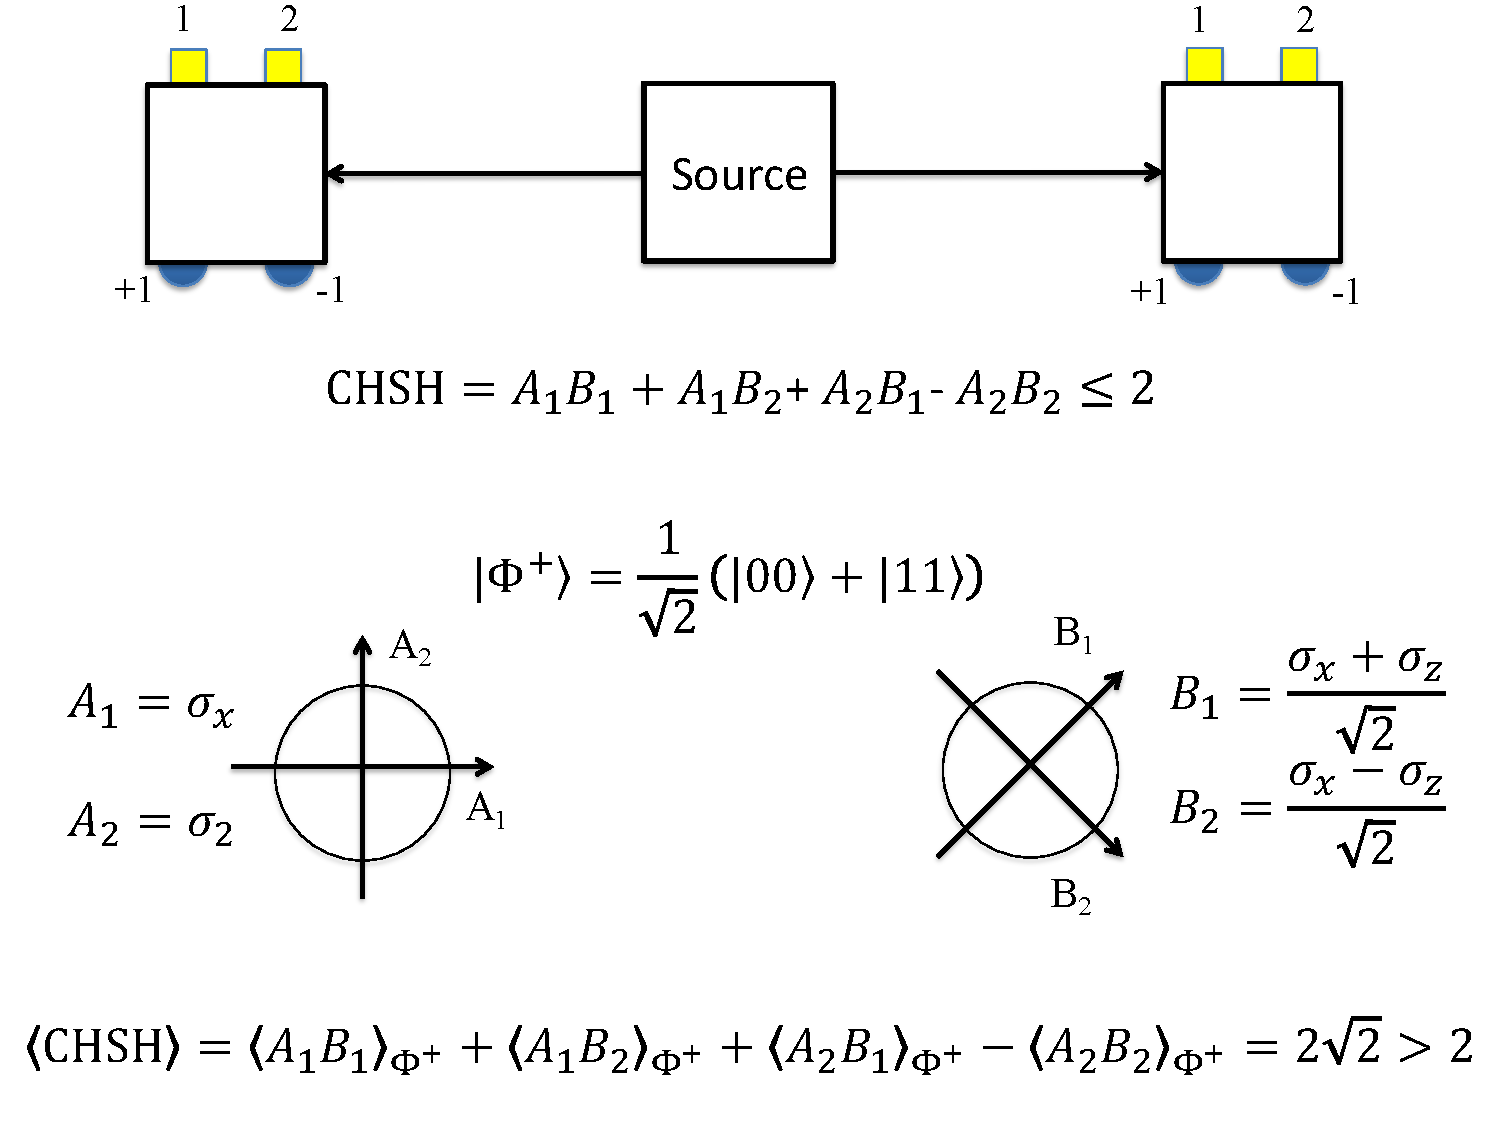
\includegraphics[width=11cm]{CHSH_Fig}\\
  \caption{\textbf{CHSH Bell inequality:} Two
  parties measure two two-outcome observables, $A_1$
  and $A_2$ for Alice, and $B_1$ and $B_2$ for Bob. The choice of
  measurement is represented by a bit, $x$ and $y$
  for Alice and Bob. The two possible
  outcomes are labeled by $\pm 1$. For the quantum violation, observables are replaced by quantum operators and they act on a two-qubit maximally entangled state.}\label{CHSHfig}
\end{center}
\end{figure}


The CHSH inequality~\cite{CHSH} is defined in the simplest Bell scenario in which the parties perform two measurements of two outputs, $m=r=2$, and the convention is to denote the performed measurement by $x,y=1,2$ and the obtained result by $a,b=\pm 1$. This convention is arbitrary but this choice simplifies the calculations. One then considers the following quantity:
\begin{equation}\label{CHSHdef}
    \text{CHSH}=A_1B_1+A_1B_2+A_2B_1-A_2B_2 ,
\end{equation}
where $A_x$ ($B_y$) denotes the measurement result by Alice (Bob) when implementing measurement $x$ ($y$). It is very simple to see that if the measurement results are deterministically fixed, that is for any assignments of $\pm 1$ to these values, the CHSH expression satisfies $|CHSH|=2$. This implies that even if the assignment changes according to a probabilistic preparation at the source $p(\lambda)$,  as in Eq.~\eqref{lrmodel}, the expectation value of this expression always satisfies
\begin{equation}\label{CHSHineq}
    \langle CHSH\rangle \leq +2.
\end{equation}
Eq.~\eqref{CHSHineq} is the famous CHSH inequality, whose mathematical derivation is astonishingly simple. The maximal violation of a inequality for LR models is called the local bound, equal to 2 for CHSH.

Let us now consider a quantum implementation of a CHSH Bell scenario in which the state prepared by the source is the two-qubit maximally entangled state 
\begin{equation}
\label{bellstate}
    \ket{\Phi^+}=\frac{1}{\sqrt 2}(\ket{00}+\ket{11}) ,
\end{equation}
and the measurement by each of the two parties are defined by the observables $A_1=\sx$, $A_2=\sz$, $B_1=(\sx+\sz)/\sqrt 2$ and $B_2=(\sx-\sz)/\sqrt 2$, see Fig.~\ref{CHSHfig}. After some calculations, it is possible to see that the quantum value of the CHSH expression for this configuration is 
\begin{equation}\label{tsirelson}
    \langle \text{CHSH}\rangle =\langle A_1B_1\rangle +\langle A_1B_2\rangle +\langle A_2B_1\rangle -\langle A_2B_2\rangle =2\sqrt 2 > 2,
\end{equation}
proving that quantum correlations do not have a description in terms of an EPR model~\eqref{lrmodel}. The value $2\sqrt 2$ is the largest possible in quantum physics and is known as the Tsirelson bound~\cite{tsirelson}.

\textbf{Exercise 1}: Compute the quantum value of each of the four terms $\langle A_x\otimes B_y\rangle$, with $x,y=1,2$, in the CHSH expression for the state~\eqref{bellstate} and settings as in Fig.~\ref{CHSHfig} and verify that they sum up to $2\sqrt 2$.



The implications of this violation are huge. First of all, there is no LR
theory able to give a value of CHSH larger than 2, so either the predictions of quantum theory are wrong or the EPR program is not possible. Bell was then able to
map all the EPR debate into a measurable condition. The only thing
left was to design the experimental situation for testing the
violation of any of these quantities. The rigorous experimental
verification of the violation of a Bell inequality came almost two
decades after Bell seminal paper~\cite{Aspect}. Since then, other
experimental tests have been performed, all in favor of the
quantum formalism~\cite{hanson,nist,vienna}.

Two facts should be mentioned here. First, note that although only
one inequality is here presented, there are many similar
conditions that characterize the set of probability distributions
achievable in a LR theory~\eqref{lrmodel}. The fact
that quantum theory predicts the existence of correlations leading to a Bell inequality violation means that these quantum correlations cannot be written in this form.
Second, despite the fact that quantum theory predicts the violation of these
inequalities, no faster-than-light communication is allowed in the
quantum formalism. This would be the case if Alice's measurement
could change Bob's measurement statistics. It is straightforward
to prove that this is not possible. Consider the situation where
Alice and Bob share a quantum state $\rho_{AB}$ on which they
apply measurements $\{M_{a|x}\}$ and $\{M_{b|y}\}$ so that
\begin{equation}
\label{qcorr}
p(ab|xy)=\tr(\rho_{AB}M_{a|x}\otimes M_{b|y}) .
\end{equation}
The probability of Alice of obtaining outcome $a$ when she measuries $x$ and Bob $y$ is
\begin{equation}
    p_A\,(a|xy)=\sum_b p\,(ab|xy)=\sum_b\tr(\rho_{AB}M_{a|x}\otimes M_{b|y})
    =\tr(\rho_{AB}M_{a|x}\otimes \one_B) =\tr(A_x\rho_A) ,
\end{equation}
where $\rho_A=\tr_B(\rho_{AB})$ and we used that $\sum_b
M_{b|y}=\one_B$ for all $y$. This means that Alice's local measurement statistics
cannot be affected by any measurement by Bob (and viceversa), as they do not depend on the implemented measurement $y$, so
no faster-than-light (in fact instantaneous) communication is possible.


\section{Quantum Cryptography}

The No-cloning Theorem shows that QIT offers new possibilities but
also limitations to the way information on quantum states can be
processed. The derivation of this theorem is astonishingly simple
and could have been found by the same fathers of quantum
mechanics. Actually, it turns out be connected to a more known
limitation of the quantum formalism: the measurement process
perturbs the state of the system. Indeed, perfect cloning would
obviously violate the fact that the state of a single quantum
system cannot be perfectly known. If perfect cloning were
possible, one could know everything of the state of a single
particle without even measuring it, just by producing clones and
measuring these, leaving the initial state untouched. On the other hand, if perfect estimation was possible, 
one could easily clone by first perfectly measuring the state and then preparing as many copies of it as desired.

Remarkably, these limitations can be converted into something
positive, as beautifully demonstrated by quantum cryptography:
since the measurement process perturbs the state of a system, the
action of any adversary trying to read quantum information propagating
through a channel has a detectable effect on the sent
state. Or in other words, the action of the adversary, also known as
eavesdropper, is limited by the impossibility of producing a
perfect copy of the quantum state. These two ideas lie at the
basis of any quantum cryptography protocol. In what follows we
present several of the main results on quantum cryptography. More
precisely, we focus all our analysis on quantum key distribution.
This is the most advanced quantum cryptography application, both
from a theoretical and experimental point of view. However, it has
to be clear that quantum cryptography is a general term that
refers to any cryptographic protocol exploiting the quantum formalism.

\subsection{One-Time Pad and Quantum Key Distribution}

Before moving into the quantum world, let us review a seminal
result by Vernam showing how to exchange private information in a
completely secure way using a pre-shared secret key.

In any cryptographic scenario, two honest parties, Alice and Bob,
want to exchange information in a private way. There is also a
third dishonest party, the eavesdropper, also called Eve, that
wants to read this information. Assume in what follows that Alice
and Bob share a secret key, that is, a list of perfectly
correlated bits which Eve has no information about. The secret
key, of length $N$, is denoted by $\vec k$, which is a string of
$N$ bits $k_i$, with $i=1,\ldots,N$. In order to send a message of
length $M\leq N$ to Bob, denoted by $\vec m$, Alice can perform
the sum modulo 2 of her message bits with $M$ secret key bits and
send the resulting $M$-bit string through the channel. More
precisely, with this operation Alice computes the boolean
XOR\footnote{The boolean XOR, denoted by $\oplus$, is the
operation such that $0\oplus 0=1\oplus 1=0$ and $0\oplus 1=1\oplus
0=1$.} of each bit in her message, $m_i$, with a bit in the secret
key, $k_i$, and sends the resulting bits, $r_i=m_i\oplus k_i$,
through the channel. It can be shown that Eve, who has access only to
the message $\vec r$ sent through the insecure channel, does not
have any information about the real message $\vec m$. However, on
Bob's side, it is very easy to decode the message due to the fact
that he knows the key. He simply has to add the received message
to his key, getting $r_i\oplus k_i=m_i\oplus k_i\oplus k_i=m_i$.
This scheme, known as the one-time pad
protocol, is secure provided that: (i) the number of key bits used
for the encoding is equal to the number of bits in the message and
(ii) the secret key bits are never reused.

The main drawback for using one-time pad is that it requires an
initially shared secret key. In a way, the problem of distributing
the message is now moved into the almost analogous problem of
distributing the key. But it is precisely here where Quantum
Mechanics can help: the distribution of a secret key can be done
in a provable secure way using quantum states and operations.
Later, this key can be employed using one-time pad to exchange the
final message in a completely secure way. The quantum protocols
allowing Alice and Bob to distribute a key in a secure way are named Quantum Key
Distribution (QKD) protocols, for obvious reasons.

\subsection{The BB84 protocol}

After introducing the idea of QKD,
we present the first protocol, introduced in 1984 by Bennett
and Brassard and known as BB84~\cite{BB84}. Recall that the goal
of the protocol is to establish a shared secret key, which is
later consumed to run one-time pad. In
the case of BB84, the key is established as follows:
\begin{itemize}
    \item Alice chooses randomly one of the four possible states
    \begin{equation}\label{bb84enc}
    \ket{\pm x}=\frac{1}{\sqrt 2}(\ket 0\pm\ket 1)\quad
    \ket{\pm y}=\frac{1}{\sqrt 2}(\ket 0\pm i\ket 1) .
\end{equation}
The bit 0 (1) is encoded onto $\ket{+x}$ and $\ket{+y}$
($\ket{-x}$ and $\ket{-y}$). The vectors $\ket{\pm x}$ and
$\ket{\pm y}$ define the so-called $x$ and $y$ basis.
    \item Bob measures randomly in one of these two bases. He
    maps his result into a classical bit using the same convention
    as Alice.
    \item Alice and Bob announce the bases used in the preparation and measurement, respectively. In
    case the bases agree, the
    outputs produced by the protocol are kept, otherwise discarded. This process is known as basis
    reconciliation.
\end{itemize}
Note that if Alice and Bob's bases agree, their bits are perfectly
correlated. On the other hand, if the bases are different, Alice's
preparation and Bob's result are completely uncorrelated. Indeed,
assume that Alice has sent $\ket{\pm x}$ and Bob measures in the
$y$ basis. He will obtain the outcome corresponding to $\ket{\pm y}$
with probability $p(\pm y|\pm x)=|\langle \pm x\ket{\pm y}|^2=1/2$. 
This is equivalent to Bob discarding Alice's state and flipping a coin.
Therefore, after the basis reconciliation, Alice and Bob discard
all the bad instances and share a list of perfectly correlated
random bits. Before proceeding, note that Alice and Bob can use any pair of bases in the Bloch sphere satisfying the previous overlap condition. The $x$ and $y$ bases appeared in the original formulation of the protocol, but one could equally formulate it using the $x$ and $z$ bases. In fact, this choice is equivalent but often simpler in terms of notation.

Let us briefly analyze why Eve cannot break this protocol. She has
to interact with the quantum particle, say a photon, encoding the
information while it propagates to Bob. The No-cloning Theorem
implies that she cannot make a perfect copy of it, forward the
first clone to Bob and keep the second one. She can however try to
measure the quantum state of the particle and read the
information. However, at this time in the protocol, she does not
know the basis chosen by Alice. Consider first that Eve measures
in the right basis. Then, she obtains all the information and can
prepare a new copy of the state to Bob. She obtains full
information about Alice's symbol and introduces no errors on Bob's
side. Now consider the case where Eve's measurement basis is
different from Alice's. Eve will obtain the right bit with
probability one half, which means that her information is zero. She now prepares a new state for Bob according to her measurement result, 
which is not equal to the one sent by Alice. Focus now on the cases where Bob's basis is the
same as Alice's (after all, these are the only cases that are kept after the
basis reconciliation process). Since Eve has prepared a ``wrong"
state, Bob will obtain the expected result with probability one
half. That is, Eve's strategy is introducing errors on Bob's side.
Alice and Bob can detect Eve's intervention by making public a
fraction of the symbols where their bases agree. If there are no
errors, it is very likely that nobody has tried to eavesdrop their
communication, and they can safely employed the remaining bits as
a secret key. If they see errors,
someone is eavesdropping the channel, so they abort. Therefore,
what BB84 prevents is that an eavesdropper reads
the key Alice and Bob are exchanging without being
detected.

It is crucial for the security of the protocol that the channel is authenticated, that is, that Alice and Bob know to communicate to each other, for instance in the process of basis reconciliation. If this is not the case, Eve could separately run the protocol with Alice and Bob, establish two different secret keys with them, and hack the a posteriori communication. Alice and Bob therefore require to authenticate their channel, which is possible if they initially share a secret key. This introduces a form of circularity in the argument, but the main point is that the amount of secret key needed to authenticate the channels can be short. Once this is done and the QKD process has started, new generated key can be used when needed for authentication.

Operationally, this description of the protocol is far from being complete. First, we have
analyzed a specific intercept and resend attack by Eve in which (i) she intercepts the sent qubits, (ii) measures them, and (iii) prepares a new state for Bob based on the obtained result. However the goal is to prove
the security of the protocol against any possible attack by Eve.
Second, from a practical point of view, it is useless to design a
protocol which is aborted whenever errors are seen. It would be
aborted in any realistic, and therefore noisy, implementation!
Fortunately, these two problems can be solved and one can design
general security proofs which are valid against any attack in a
noisy situation. In fact, the scope of a security proof is to show how Alice and Bob can distill a secret key in the presence of errors. 
We present the main ideas to build a general
security proof for QKD protocols below. But first,
we discuss other examples of protocols, showing that many variants are possible.

\subsection{Other protocols}

The BB84 protocol distributes a secret key from Alice and Bob
using quantum states that are prepared by Alice, sent through the
insecure channel and measured by Bob. This type of protocols are
known as \emph{prepare and measure}. Clearly, the construction is much more
general and one can design many other protocols for secure key
distribution based on this idea. The main purpose of this section
is to present some of them. Actually, one can find many QKD
protocols in the literature. Here, we choose those that represented
an important theoretical advance.

\subsubsection{B92}

The main reason why Eve cannot read the information 
encoded on the sent quantum states is that Alice is choosing them from a set that contains non-orthogonal quantum states.
Being non-orthogonal, Eve cannot clone or measure all of them
without introducing detectable errors. In 1992, Bennett showed that two non-orthogonal states
are enough for secure QKD~\cite{B92}. The interest of this protocol comes from
the fact that it is the one involving the minimal number of prepared states, namely two.

The protocol works as follows. Alice encodes a random bit into two non-orthogonal states, $\ket{\psi_0}$ and $\ket{\psi_1}$, and sends the prepared state to Bob through the insecure channel. Again, Eve's attack is limited by the non-orthogonality of the states. A possible simple measurement by Bob is as follows: he randomly chooses to measure in the basis defined by $\ket{\psi_0}$ and its orthogonal state, denoted by $\ket{\psi^\perp_0}$ and such that $\langle \psi^\perp_0\ket{\psi_0}=0$, or the basis $\{\ket{\psi_1},\ket{\psi^\perp_1}\}$. When Bob gets the output corresponding to any of the orhogonal states for any of the two measurements, say outcome corresponding to $\ket{\psi^\perp_0}$ when measuring $\{\ket{\psi_0},\ket{\psi^\perp_0}\}$, he knows that the state was for sure not $\ket{\psi_0}$ because $\langle \psi^\perp_0\ket{\psi_0}=0$, and hence it has to be $\ket{\psi_1}$. Therefore, in this reconciliation, Bob announces those instances in which his measurement gave an outcome corresponding to any of the states orthogonal to those prepared by Alice. A more efficient but also experimentally demanding measurement is given by the one attaining the optimal unambiguous discrimination of the states $\ket{\psi_0}$ and $\ket{\psi_1}$. 

\textbf{Exercise 2: Unambiguous discrimination of two non-orthogonal pure states.} Consider two non-orthogonal pure states $\ket{\psi_0}$ and $\ket{\psi_1}$, with $\langle \psi_0\ket{\psi_1}>0$. Without loss of generality, the two states can be rotated to be in the $XZ$ plane and with the $+z$ axis as bisector, so that they read:
\begin{equation}
\label{states}
\ket{\psi_0}=\left(\begin{array}{c}\cos\theta \\ \sin\theta\end{array}\right) \quad\quad
\ket{\psi_1}=\left(\begin{array}{c}\cos\theta \\ -\sin\theta\end{array}\right) ,
\end{equation}
with $0\leq\theta\leq\pi/4$. Let $\ket{\psi}$ be an unknown state chosen between these two with equal probability. Consider a three-outcome measurements defined by the operators:
\begin{equation}
\label{povm}
M_0=\mu\proj{\psi_1^\perp} \quad\quad  M_1=\mu\proj{\psi_0^\perp}   \quad\quad  M_?=\one-M_0-M_1 ,
\end{equation}
where $\ket{\psi_i^\perp}$ denotes the state orthogonal to $\ket{\psi_i}$. 
\begin{itemize}
\item[a)] Find the range of values of $\mu$ so that the measurement is well defined, that is, all the three measurement operators are positive semi-definite. 
\item[b)] For this value of $\mu$, compute the probabilities of obtaining the three outputs for each of the two states. What's the operational meaning of this three-outcome measurement? 
\item[c)] Finally, determine the value of $\mu$ that minimises the average probability of obtaining the third outcome, that is:
\begin{equation}
P_?=\frac{1}{2}\left(p(?|0)+p(?|1)\right) .
\end{equation}
How does it relate to the overlap between the two states?
\end{itemize}


\subsubsection{Six-state protocol}

The six-state protocol, introduced by Bru{\ss}~\cite{6state}, 
goes in the opposite direction: it involves more states to make
Eve's attack more difficult. In the BB84 protocol, only four states
belonging to a given equator in the Bloch sphere, say the plane
$xy$, are used. However, one could consider more elaborated
protocols in which Alice prepares states that are better
distributed over the sphere. This is precisely the main idea
behind the six-state protocol: Alice prepares a state from the
six-state set $\{\ket{\pm x},\ket{\pm y},\ket{\pm z}\}$. Bob now
measures along these three bases, $x$, $y$ and $z$. Clearly, after basis reconciliation,
Alice and Bob are assumed to derive a list of perfectly correlated
bits. From Eve's point of view, her task becomes more complex as
she has to clone, or distinguish, among more non-orthogonal
states. However, from Alice and Bob's point of view, only 1/3 of the rounds are kept after basis reconciliation. 
After all, the improvement in security is moderate, while in some implementations the technological
requirements to prepare the six states are more demanding, so the protocol has hardly been adopted in practice.

\subsubsection{Goldenber-Vaidman protocol}

The last protocol that we present in this part was introduced by
Goldenber and Vaidman~\cite{vaidman}. The protocol uses entanglement and proved that secure key
distribution is still possible using two orthogonal states if
these two states are used in a careful way. The idea of the
protocol is as follows: Bob prepares a two-qubit maximally
entangled state, $\ket{\Phi^+}=(\ket{00}+\ket{11})/\sqrt 2$. He
sends only one of the particles to Alice. Alice now applies nothing, that is $\one$,
or $\sigma_z$ depending on the bit she wants to transmit, and sends
the qubit back to Bob. The two states, depending on Alice's random
bit, are $\ket{\Phi^\pm}$, where now $\ket{\Phi^-}=(\ket{00}-\ket{11})/\sqrt 2$. On reception, Bob
can perfectly discriminated between these two states and read the result because they are orthogonal.
Although, as said, the information encoding by Alice produces two
orthogonal states, this fact cannot be exploited by Eve. She has
only access to one of the two
quantum particles prepared and transmitted  by Bob, while the other particle always remains on
Bob's lab, hence never accessible to Eve. This makes the quantum measurement by Eve on the two
orthogonal states impossible. In fact, the qubit Eve can access to is always in the reduced state of $\ket{\Phi^\pm}$, equal to $\one/2$ for both states, which guarantees the protocol security.

\subsection{Ekert protocol}

In all the previous protocols, except the last one, entanglement
does not play any role: Alice prepares single-particle states
that are sent to and measured by Bob. In 1991, Artur Ekert proposed
a novel scheme for secure QKD that was based on entangled states
and a Bell inequality violation~\cite{Ekert}. Ekert was not aware of
the previous work by Bennett and Brassard, which appear in the
proceedings of a computer scientist conference. Actually, he
(re)discovered QKD in an independent way. However his approach to
the problem seemed to be completely different, based on the
Bell inequality violations produced by entangled states rather the the
non-orthogonality of quantum states.

The protocol by Ekert works as follows (we provide here a slightly
different version of his original protocol which is simpler but
conceptually equivalent): Alice and Bob receive correlated quantum
bits assumed to be in a maximally entangled state, say the state~\eqref{bellstate}. 
Alice and Bob apply each the two measurements $A_1$,
$A_2$ and $B_1$ and $B_2$ given in Fig. \ref{CHSHfig}, which
maximise the value of the CHSH inequality. Moreover Alice applies
a third measurement $A_3$ in the same direction as one of the
measurements by Bob, say $B_1$, to get perfectly correlated
outcomes. The idea is that the honest parties obtain a key from
$A_3$ and $B_1$, which are perfectly aligned, while compute the
CHSH value to guarantee that they share a maximally entangled state. In the ideal
case, this parameter should be equal to $2\sqrt 2$.

The intuition is that if the measurements by Alice and Bob lead to
a Bell inequality violation, there is no hidden-variable model
reproducing the outcomes. This absence of hidden-variable model
should guarantee the privacy of the obtained outcomes. In other
words, if Eve could predict the outcomes by the honest parties,
this would constitute a local hidden variable model for the
experiment. However this is impossible because the observed data
violate a Bell inequality violation. Clearly, this is only the
intuitive argument that led Ekert to the construction of this
protocol, but does not represent any security proof. 

\subsection{Bennett-Brassard-Mermin argument}

A few months after Ekert work, Bennett, Brassard and
Mermin~\cite{BBM} wrote an article showing that a QKD protocol \`a
la Ekert can always be transformed into an equivalent protocol
without entanglement, \`a la BB84, where states are prepared by
Alice and measured by Bob. Their argument goes as follows.

First of all the role of a Bell inequality violation in Ekert's
proposal is to certify that Alice and Bob share a two-qubit
maximally entangled state. However, there are other measurements
which can provide the same level of certification. For instance,
it is the only state which gives perfect correlations when both
local parties measure in the $x$ and $z$ basis. That is, it is the
only two-qubit state such that
$\bra{\psi}\sigma_x\otimes\sigma_x\ket{\psi}=
\bra{\psi}\sigma_z\otimes\sigma_z\ket{\psi}=1$. Thus, the detection of the maximally entangled state
can equally be performed via a protocol in which
both Alice and Bob measure in the $x$ and $z$ basis. Note that now
Alice does not need to introduce a third basis to get outcomes
that are perfectly correlated to Bob's.

The remaining step is noting that when measuring her quantum
particle, Alice is effectively preparing a state for Bob. Indeed,
in the ideal case, Alice receives half of a maximally entangled
state. Then, one can see that her measurement projects Bob's
particle into a state which is equal to the measurement result by
Alice. This follows from the simple observation that:
\begin{eqnarray}
% \nonumber to remove numbering (before each equation)
  _A\bra{\pm x}\ket{\Phi^+}_{AB} &=& \frac{1}{\sqrt 2}\ket{\pm x}_B \nonumber\\
  _A\bra{\pm z}\ket{\Phi^+}_{AB} &=& \frac{1}{\sqrt 2}\ket{\pm
  z}_B .
\end{eqnarray}
That is, depending on her choice of basis, Alice is preparing a
state in the plus or minus direction with probability equal to
1/2. Clearly, the resulting protocol is equivalent to the original
protocol in terms of security. But the resulting protocol is
nothing but the original BB84 protocol and does not require any
entanglement. Thus, the authors of Ref.~\cite{BBM} concluded that
the approach by Ekert did not provide any new significant insight
into the problem of QKD, because both approaches were equivalent.

Apart from the conceptual implications, the work by Bennett,
Brassard and Mermin was also important from a technical point of
view, as it pointed out a nice correspondence between entanglement-based
\`a la Ekert and prepare-and-measure protocols \`a la BB84. On the one hand, most of
the protocols based on entanglement can be mapped into an
equivalent prepare-and-measure protocol using the previous
ideas. On the other hand,
any prepare-and-measure protocol can be mapped into an equivalent
entanglement-based protocol. Indeed, assume that in the initial
prepare-and-measure protocol Alice prepares the states
$\{\ket{\psi_i}\}$ with probabilities $p_i$. This can be done by
Alice by preparing an entangled state
\begin{equation}
    \sum_i \sqrt{p_i}\ket{i}_A\otimes\ket{\psi_i}_B ,
\end{equation}
and measuring now her particle in the basis $\{\ket{i}\}$. 
As we discuss in the next section, this parallelism provides an
important conceptual and technical simplification of security
proofs in QKD. Usually, the security  proofs of QKD protocols are derived in the 
entanglement-based scenario, because there it is simpler to construct them, but the prepare-and-measure equivalent version is implemented in practice, as it just involves the preparation single-particle states and measurements.

\section{General structure of QKD protocols}

The general structure of a QKD protocol is as follows:
\begin{enumerate}
    \item Repeat $N$ times: Alice prepares states $\ket{\psi_a}$ with probability $p_a$ and sends them to Bob through the insecure channel. Bob performs one of the measurements $M_j$ with probability $p_j$ on the received particle, obtaining the result $r$. After this process Alice and Bob have a list of $N$ symbols corresponding to the prepared states on Alice's side $\vec a=(a_1\ldots a_N)$ and implemented measurement on Bob's side $\vec b=(b_1\ldots b_N)$. Note that here we have combined the chosen measurement by Bob $j$ and the obtained result $r$ within $b$, that is $b=(j,r)$.
    \item Alice and Bob announce the prepared state and performed measurement and result for $n$ of these rounds. This allows them to estimate the frequencies of obtaining result $r$ when performing measurement $j$ on state $\ket{\psi_i}$.
    \item Using this information, and the security proof, Alice and Bob know how to process their classical list of symbols $\vec a$ and $\vec b$ to distill a secret key rate of length $K$, $\vec k=(k_1\ldots k_K)$. The length of this key depends on the previous estimation round. If the channel quality is too bad, Alice and Bob conclude that no key distillation is possible, $K=0$, and the protocol is aborted. 
\end{enumerate}
Several remarks are important here:
\begin{itemize}
\item In principle, the larger the number of rounds $N$, the better the protocol performance: it reduces the statistical fluctuation when estimating the properties of the channel and therefore Alice and Bob have a much more precise understanding of the key distillation process. In the limit of $N\rightarrow\infty$, one can define the key rate $k=\lim_{N\rightarrow\infty} K/N$.
\item The number of rounds $n$ should be sufficient to achieve a reliable estimation of the channel properties, that is, to accumulate enough statistics so that these properties are determined with a given pre-determined confidence. But, to optimise the protocol performance, it should not be much larger than this, as these rounds do not contribute to the secret key. In the limit of large $N$, one can have very large values of $n$, and therefore an arbitrarily good estimation of the channel properties, but such that $n\ll N$. In other words, the estimation hardly affects the asymptotic key rate.
\item The security proof, discussed below, is crucial in step 3 to understand how Alice and Bob should distill the key from the noisy list of symbols $\vec a$ and $\vec b$.
\end{itemize}
In the case of BB84, $a=(b_A,p)$, where $b_A$ specifies Alice's choice of basis and $p$ the prepared element of the basis, so that $a$ can be equal to $(z,\pm 1)$ or $(x,\pm 1)$. These four states are prepared with the same probability equal to $1/4$. On Bob's side, we can also write $b=(b_B,r)$, where $b_B$ now denotes Bob's choice of basis. The basis reconciliation process in which Alice and Bob only keep those symbols where $b_A=b_B$ is part of the key distillation process in step 3 mapping the initial list of symbols obtained in step 1 into the final key.

The protocol in the entanglement picture is very similar, but step 1 is now replaced by 
\begin{enumerate}
    \item Repeat $N$ times: Alice prepares the state $\ket{\Psi}_{AA'}=\sum_a \sqrt{p_a}\ket a_A\otimes\ket{\psi_a}_{A'}$, where $\{\ket{a}\}$ defines an arbitrary basis in system $A$. She measures system $A$ in this basis getting result $a$ with probability $p_a$. She then sends system $A'$, which is in state $\ket{\psi_a}$, to Bob through the insecure channel. Bob performs one of the measurements $M_j$ with probability $p_j$ on the received particle, obtaining the result $r$. After this process Alice and Bob have a list of $N$ symbols corresponding to the measurement result on Alice's side $\vec a=(a_1\ldots a_N)$, and implemented measurement on Bob's side $\vec b=(b_1\ldots b_N)$. Note that here we have combined the chosen measurement by Bob $j$ and the obtained result $r$ within $b$, that is $b=(j,r)$.
\end{enumerate}
In the particular case of BB84, the four states can be grouped into two bases. This simplifies the entanglement-based equivalent protocol, which, as said, can be seen as measuring bases $x$ and $z$ on half of a maximally entangled state. However, grouping the prepared states into more than one basis is in general not possible, e.g. for the B92 protocol.

\section{Security proofs}

The previous sections have summarised some of the most known
protocols for secure QKD and concluded with their general structure. The intuition for all of them is that
an attack by Eve introduces detectable errors in the channel. 
The intuitive argument then goes on by saying that Alice and Bob can monitor the
presence of these errors and stop the protocol aborting the
eavesdropping attack. Clearly, while this intuition suggests that
the scheme may be secure, it is unacceptable when dealing with
practical implementations. In any realistic scenario, there will
be errors which are not due to Eve but just a consequence of noise
in the channel and/or imperfections on Alice and Bob's labs.
Therefore, we cannot accept that Alice and Bob abort the protocol
whenever they observe errors.

The purpose of a security proof is to deal with a noisy scenario
and make QKD protocols implementable in practice. The main idea is
that Alice and Bob should conclude from the amount of observed
errors whether they are able to establish a secret key. The reason
why they can do that is because in quantum theory it is
possible to put a bound on the information Eve has access to from
the amount of error (or correlations) between Alice and Bob. If
Alice and Bob have a small amount of errors error (large correlations), Eve has little
information. A security proof makes this trade-off quantitative.

In what follows we sketch the main steps in a
security proof. Our purpose is not to provide a detailed
derivation of these proofs, as they are usually quite technical
and involved, but to point out the main ideas and results used in
their derivation.

\subsection{Eve's attacks}

We first describe the possible attacks that Eve can implement. 
As an illustration, we consider a paradigmatic attack on BB84 based on what are called optimal cloning machines. This is an example of a general family of attacks called \emph{individual} in which: (i) Eve intercepts the particle sent from Alice to Bob, $\ket{\psi_a}$; (ii) adds another particle in a reference state, say $\ket 0$, and performs a unitary operation $U_E$ on the two particles; (iii) Eve forwards one of the resulting states to Bob, while she keeps the other particles in a quantum memory; (iv) once the bases are announced by the honest users, Eve measures her particle, see Fig.~\ref{indattacks}, getting the measurement result $e$. As a result of this process, Alice, Bob and Eve share correlated random variables corresponding to their prepared states and measurement results, $a$ and $b$ for the honest users, and $e$ for Eve, described by the probability distribution $P(a,b,e)$.

\begin{figure}
\begin{center}
  % Requires \usepackage{graphicx}
  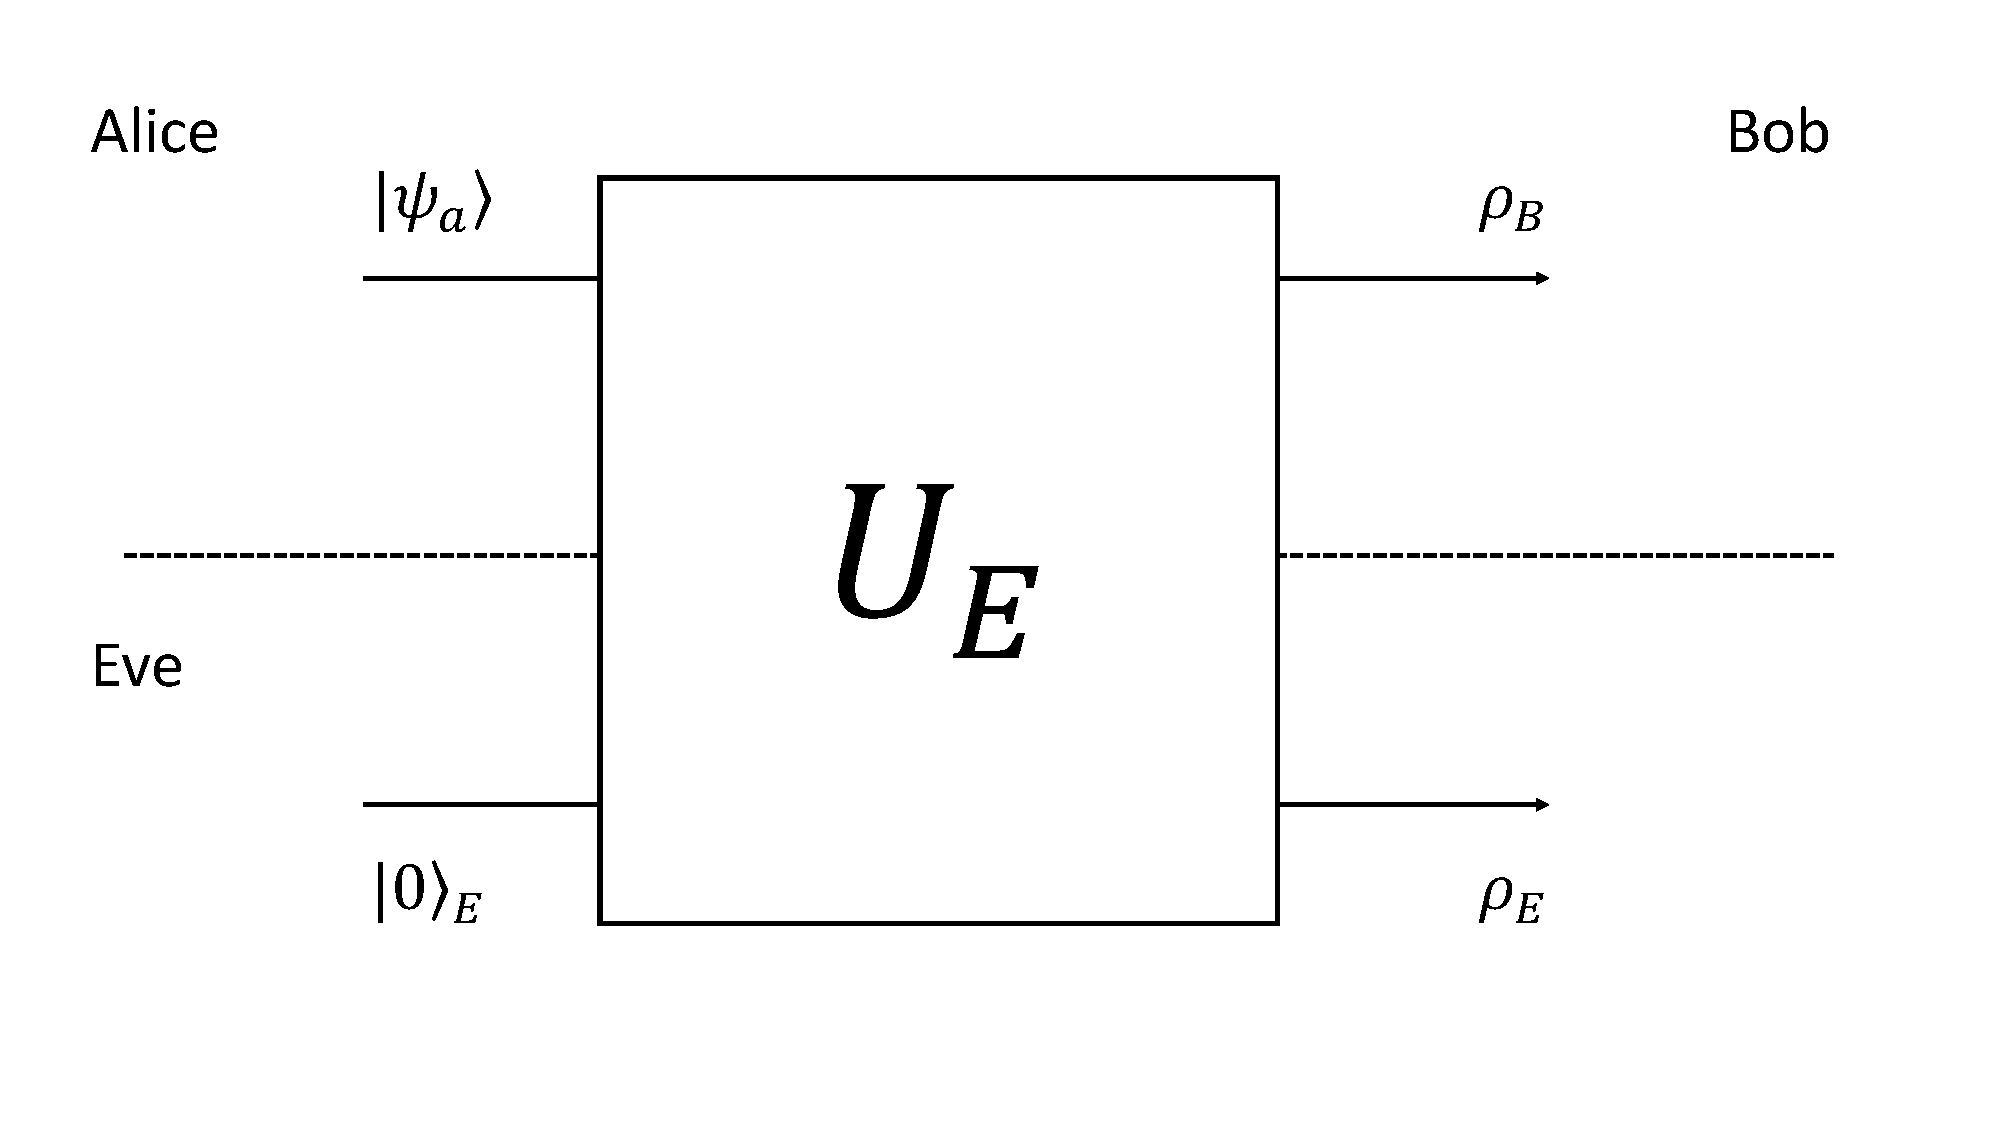
\includegraphics[width=10cm]{Cloning_Attack.pdf}\\
  \caption{\textbf{Structure of individual attacks:} Eve interacts with the states prepared by Alice and a reference state, say $\ket 0$ through a unitary operation $E_E$. She forwards one particle to Bob and keeps the other one, which is measured after the bases are announced.}\label{indattacks}
\end{center}
\end{figure}


\textbf{Exercise 3}: Consider a cloning individual attack in which Eve's action is described by a one-parameter family of unitary operations $U(\eta)$. While the no-cloning theorem states that an unknown quantum state
cannot be cloned, approximate cloning is always possible.
Consider states in the equator of the Bloch sphere, that is,
\begin{equation}\label{thetast}
    \ket{\theta}=\frac{1}{\sqrt
    2}\left(\ket{0}+e^{i\theta}\ket{1}\right) .
\end{equation}
Note that if $\theta=0,\pi/2,\pi,3\pi/2$ one gets the four states $\ket{\pm x}$ and $\ket{\pm y}$ that can be used for BB84. Take a generic state $\ket{\theta}$ and an ancillary state
$\ket{0}$ and apply the global transformation (acting on the two
states) $U(\eta)$, or $U$ to simplify the notation, 
\begin{eqnarray}
% \nonumber to remove numbering (before each equation)
  U\ket{00} &=& \ket{00}\,, \nonumber\\
  U\ket{10} &=& \cos\eta\ket{10}+\sin\eta\ket{01} .
\end{eqnarray}
\begin{itemize}
\item[a)] Briefly explain why $U$ is a valid unitary transformation on the considered quantum states.
\item[b)] Compute the final two-qubit state $\ket{\psi(\theta)}_{BE}=U_{BE}\ket{\theta}_B\ket{0}_E$
and the reduced states $\rho_B$ and $\rho_E$, where
$\rho_B=\tr_E\proj{\psi(\theta)}$ and similar for $\rho_E$.
\item[c)] Compute the overlap, or fidelity, of these two states with the initial
state, that is $F_i=\bra{\theta}\rho_i\ket{\theta}$, with $i=B,E$.
Do these fidelities depend on $\theta$? Find also the value of
$\eta$ for which the two fidelities become equal. Finally, compute the
reduced states when $F_B=1$. How do you interpret these results?
\item[d)] Apply this attack to the BB84 protocol when Alice and Bob use the states $\ket{\pm x}$ and $\ket{\pm y}$ and Eve measures in the same basis as Alice and Bob after basis reconciliation. Compute the distribution of variables $P(a,b,e)$ where $a$ denotes the bit encoded by Alice, and $b$ and $e$ the measurement results by $e$. Compute also the so-called Quantum Bit Error Rate (QBER) defined by the probability that Bob's result is different from Alice's preparation when the bases agree, and the mutual information between Alice and Bob, $I(A:B)$, and between Alice and Eve, $I(A:E)$, where $I(X:Y)=H(A)+H(B)-H(AB)$ and $H(X)=-\sum_x p(x)\log(p(x))$.
\end{itemize}

Historically, individual attacks were the first studied in the security of cryptographic protocols. The previous cloning attack is optimal in terms of fidelities because, for a given fidelity on Bob's side, $F_B$, optimises the value of $F_E$. Individual attacks, however, are not the most general because assume that Eve (i) interacts in the same way with all the quantum particles sent from Alice to Bob and (ii) measures her particle at the end of basis reconciliation. Individual attacks may for instance miss the possibility that a correlated interaction among rounds of the protocol could give Eve more information, or that Eve could wait until the end of the key distillation process and use all the information revealed during it to optimise her measurement, or even wait until the key is used. In fact, the security proof should work for the most general situation in which Eve keeps her quantum particle in a quantum memory and does not measure it: if one proves security for this situation, the proof also holds for any measurement Eve could later apply to her quantum system. Individual and the most general attacks are shown in Fig.~\ref{attacks}, where we show them in the entanglement-based picture usually employed to prove security. An intermediate attack that happens to be very useful is the so-called \emph{collective} attack in which Eve (i) keeps her information in a quantum form, that is, stores her quantum particles in a memory, but (ii) she applies the same interaction in each round. 

Finally, since in the most general situations we are considering attacks in which Eve keeps her information in a quantum form, the definition of secret key should be adapted to this scenario. Informally, a protocol is able to distill a key of lenght $k$, whenever the result of the protocol is a state $\rho_{ABE}$ that is very close to the ideal state
\begin{equation}
\label{secretkey}
\rho_{ABE}^{(k)}=\frac{1}{2}(\proj{00}+\proj{11})_{AB}^{\otimes k}\otimes\proj{E}_E ,
\end{equation}
that is, Alice and Bob share $k$ perfectly correlated bits that are secret, because uncoupled from Eve's quantum system, in an arbitrary reference state $\ket E$.


\begin{figure}
\begin{center}
  % Requires \usepackage{graphicx}
  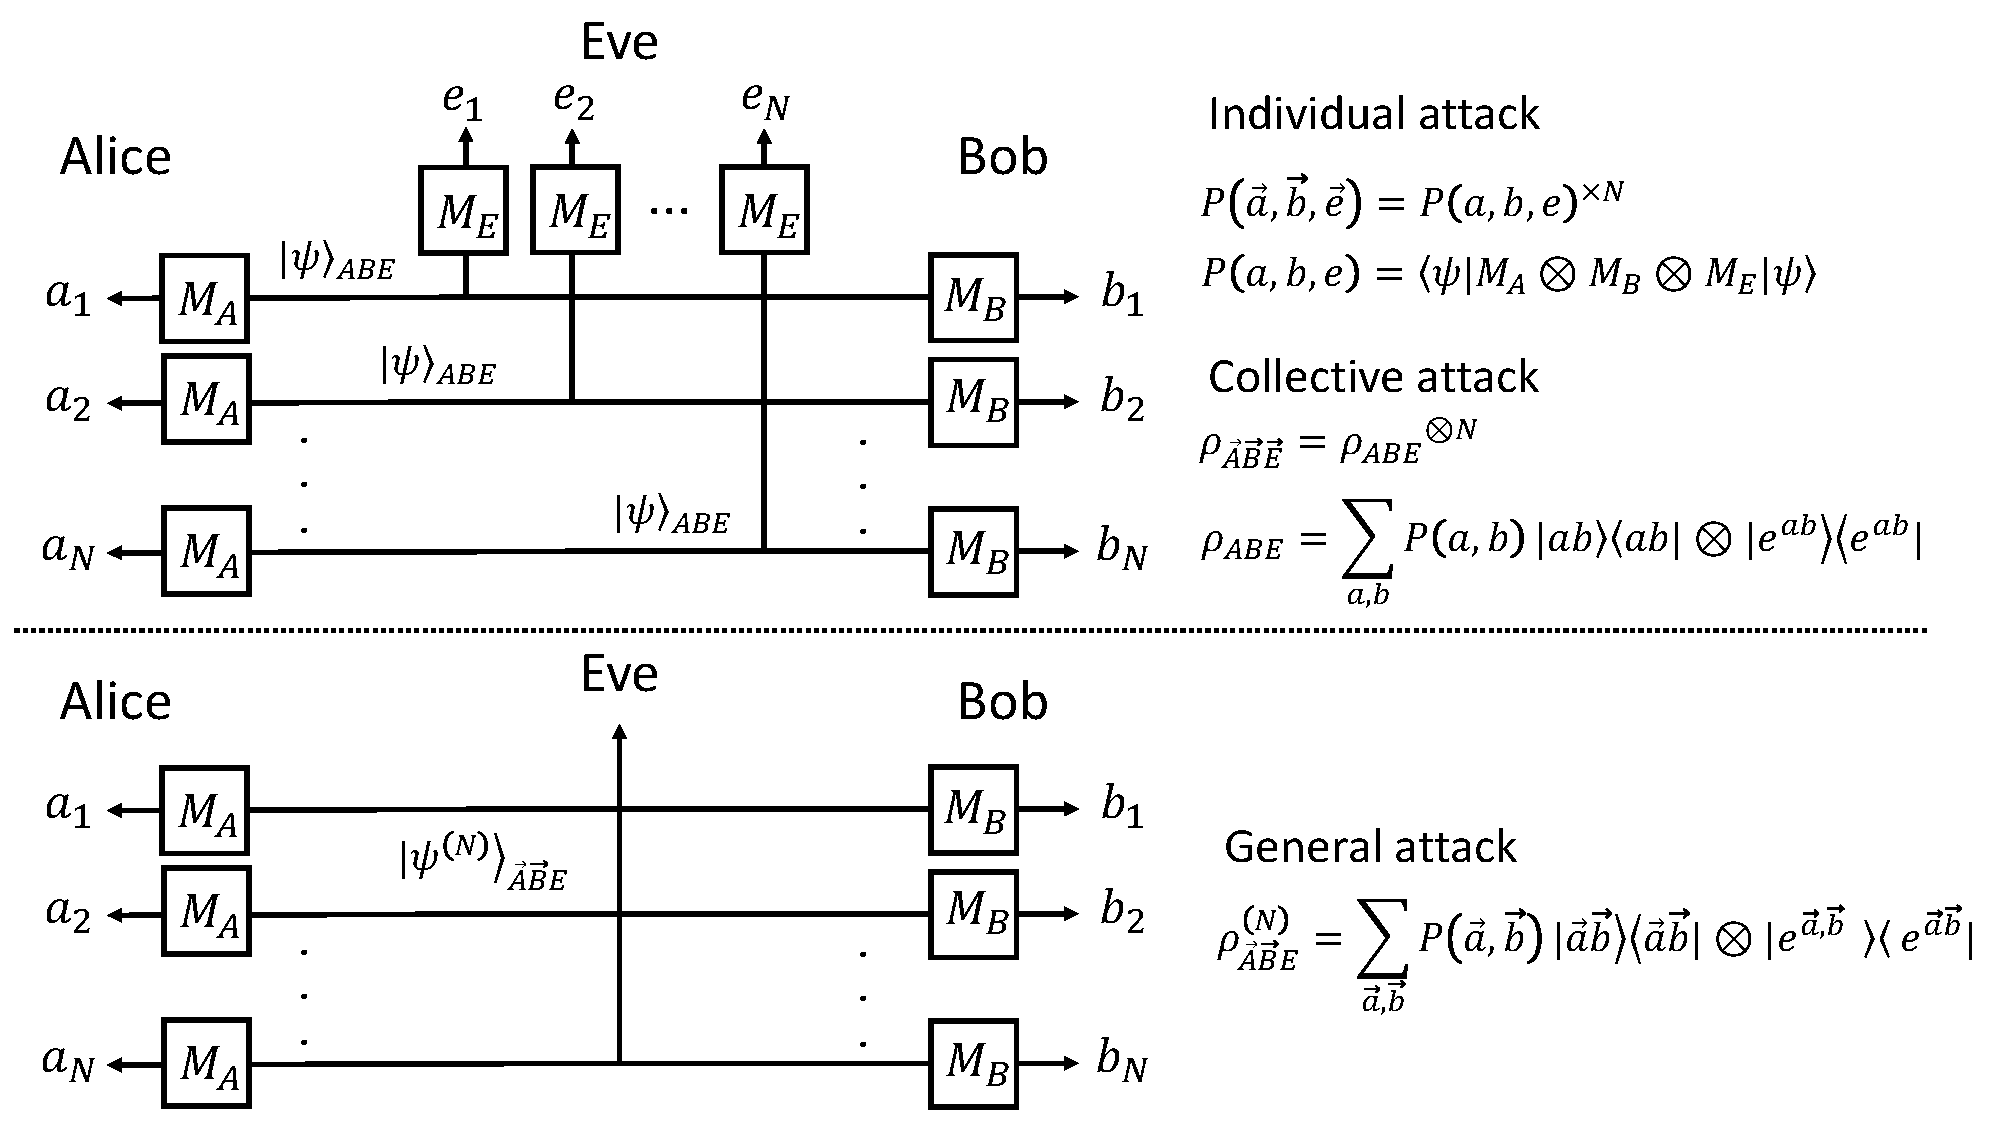
\includegraphics[width=13cm]{attacks.pdf}\\
  \caption{\textbf{Structure of eavesdropping attacks:} In the individual and collective attacks, Eve prepares $N$ copies of the same state $\ket{\psi}_{ABE}$ and forwards a particle from each state to Alice and Bob who measure them. In the case of individual attacks, Eve also applies the same measurement on each particle after basis reconciliation. In collective attacks, Eve keeps her $N$ quantum systems in a quantum memory for later use. In general attacks, Eve prepares a joint state $\ket{\psi^{(N)}}_{\vec A\vec BE}$, forwards the corresponding particles to Alice and Bob for their measurements, while she keeps a (possibly large) quantum system in a quantum memory. All the attacks are shown in the entanglement-based scenario.}\label{attacks}
\end{center}
\end{figure}


\subsection{Key rate for collective attacks} 

The importance of studying collective attacks comes from a result by Renner~\cite{renner} who proved that by increasing the number of protocol rounds $N$, 
and for a large family of protocols, that includes all those described here, the amount of key that can be distilled in a protocol against general attacks tends to the key rate that can be distilled against the optimal collective attack. In other words, the length of secret key $K$ that can distilled after $N$ rounds satisfies $\lim_{N\rightarrow\infty} K/N=k_C$, where $k_C$ is the key rate against collective attacks. For a practical realisation with a finite number of rounds, there will be corrections to this limit and $k_C$ cannot be attained, as one has $K=k_CN-o(N)$. These corrections are relevant in practical situations and a full security proof is able to compute, or bound them. But $k_C$ is the asymptotically attainable rate. 

Putting everything together, in the entanglement-based picture, the security analysis of a protocol under collective attacks is as follows:
\begin{itemize}
    \item For all the rounds of the protocol, Eve prepares the tripartite pure state $\ket{\Psi}_{ABE}$, unknown to Alice and Bob, and distributes particles $A$ and $B$ to the honest users, while she keeps $E$ in a quantum memory. The reduced state shared between Alice and Bob is $\rho_{AB}=\tr_E\proj{\Psi}_{ABE}$.
    \item Alice (Bob) chooses to perform a series of measurements  $M_{a|x}$ ($M_{b|y}$)
    on her (his) particles, where $x$ ($y$) denotes the implemented measurement and $a$ ($b$) the obtained result, with probabilities $p_A(x)$ ($p_B(y)$).
    \item From their measurement results, Alice and Bob can estimate $p(ab|xy)=\tr(\rho_{AB}M_{a|x}\otimes M_{b|y})$. These probabilities fully or partly characterize their shared state. We denote by $\mathcal{S}_{AB}$ the set of states between Alice and Bob compatible with the observed probability distributions $p(ab|xy)$. 
    \item For each of these states $\tilde\rho_{AB}\in\mathcal S_{AB}$, Alice and Bob can include Eve
system because of the Schmidt
decomposition. Indeed, consider the spectral decomposition of
$\tilde\rho_{AB}$, namely $\tilde\rho_{AB}=\sum_i\lambda_i\proj{\lambda_i}$.
If Alice and Bob want to include Eve in the picture, they should
characterise those pure states $\ket{\tilde\Psi}_{ABE}$ compatible with their shared state $\tilde\rho_{AB}$. Any such state can be written as
\begin{equation}\label{psiabe}
    \ket{\tilde\Psi}_{ABE}=\sum_i
    \sqrt{\lambda_i}\ket{\lambda_i}_{AB}\ket{e_i} ,
\end{equation}
where $\{\ket{e_i}\}$ define an orthonormal basis in Eve's space.
Note that Eve's dimensional space is equal to the rank (number of
non-zero eigenvalues) of $\tilde\rho_{AB}$. Given
$\ket{\tilde\Psi}_{ABE}$, which is completely specified by the basis
$\{\ket{e_i}\}$, any other state $\ket{\Phi}_{ABE}$ compatible with $\rho_{AB}$
is such that
$\ket{\Phi}_{ABE}=\one_{AB}\otimes U_E\ket{\tilde\Psi}_{ABE}$. That is,
the only difference between these two states is a unitary
operation on Eve's space, which corresponds to a different basis
$\{\ket{e'_i}\}$. This implies that any of these states is equally
powerful from Eve's point of view. We denote by $\mathcal{S}_{ABE}$ the set of pure states between Alice, Bob and Eve compatible with the observed probability distributions $p(ab|xy)$. Of course the state $\ket{\Psi}_{ABE}$ actually prepared by Eve is an element of this set.
\item Alice and Bob focus on those measurements that are used to construct the key, for instance measurements $z$ by Alice and Bob in the BB84 protocol. When they apply these measurements to any of the states $\ket{\tilde\Psi}_{ABE}$, one gets
\begin{equation}\label{ccq}
    \tilde\rho_{ABE}=\sum_{a,b}p(ab)\proj{a}_A \otimes\proj{b}_B\otimes\proj{\tilde e^{ab}}_E
    ,
\end{equation}
where $p(ab)=\bra{ab}\tilde\rho_{AB}\ket{ab}$ is the probability of
getting outcomes $a$ and $b$ and $\ket{\tilde e^{ab}}$ is Eve's projected
state when Alice and Bob have got these results. Up to normalization, this state is proportional to
\begin{equation}\label{evestate}
    \ket{\tilde e^{ab}}\propto\langle ab\ket{\tilde\Psi}_{ABE} .
\end{equation}
More precisely, the pure state $\ket{\tilde e^{ab}}$ is given by the right-hand side of the previous equation after normalisation.
The state \eqref{ccq} is often said to contain
classical-classical-quantum (ccq) correlations. In fact, note that, although
the state is given in a quantum form, Alice and Bob share only
classical outcomes whose correlations are encapsulated by the
probability distribution $p(ab)$. On Eve's side, however, she has
a quantum state $\ket{\tilde e^{ab}}$ that depends on, or equivalently, is correlated to Alice and Bob's classical
measurement results.
\item Devetak and Winter proved that the key rate distillable $k_C$ from an asymptotically large number of identical copies of a ccq state~\eqref{ccq} is lower bounded by the so-called Devetak-Winter bound, which reads~\cite{dwrate}
\begin{equation}\label{dwbound}
    k_C\geq K_{DW}(\tilde\rho_{ABE})=I(A:B)-\chi(A:E) .
\end{equation}
Clearly, the bound is a function of the ccq state $\tilde\rho_{ABE}$.
Recall that $I(A:B)=H(A)+H(B)-H(A,B)$ is the mutual information of the
probability distribution $p(ab)$. The expression $\chi(A:E)$ denotes the
Holevo quantity\cite{Holevo} for the effective coding of Alice's measurement
outcome $a$ on Eve's quantum states. Indeed, any measurement result by
Alice projects Eve's state into
\begin{equation}
    \tilde\rho_E^a=\tr_{AB}(\proj a\otimes\one_{BE}\proj{\tilde\Psi}_{ABE})/p(a),
\end{equation}
where $p(a)$ is the probability that Alice observes the result $a$, $p(a)=\sum_bp(ab)=\tr(\proj a \otimes \one_{BE}\proj{\Psi}_{ABE})=\tr(\proj a\otimes\one_B\rho_{AB})=\tr(\proj a\rho_A)$, where $\rho_A=\tr_B\rho_{AB}$.
The Holevo quantity then reads
\begin{equation}
    \chi(A:E)=S(\tilde\rho_E)-\sum_a p(a)S(\tilde\rho_E^a) ,
\end{equation}
where $\tilde\rho_E=\sum_a p(a)\tilde\rho_E^a=\tr_{AB}\proj{\tilde\Psi}_{ABE}$. 
To compute a valid bound on the the key rate, Alice and Bob should minimise the Devetak-Winter bound over all those states compatible with the observed statistics
\begin{equation}\label{dwbound}
    k_C\geq \min_{\tilde\rho_{ABE}\in\mathcal S_{ABE}}K_{DW}(\tilde\rho_{ABE}) .
\end{equation}
In fact, Alice and Bob should assume that the prepared state by Eve is the worst possible, that is, the solution to the previous minimisation problem. This minimisation provides the searched asymptotic key rate.
\end{itemize}

\textbf{Exercise 4: Computation of key rates.} In the six-state protocol, Alice prepares the eigenstates of $\sigma_x$, $\sigma_y$ and $\sigma_z$, and sends them to Bob, who measures these observables. After basis reconciliation, Alice and Bob keep only those cases in which they use the same basis. In the entanglement-based picture, the protocol is basically equivalent to the preparation of the two-qubit maximally entangled state~\eqref{bellstate} on which Alice and Bob measure the three Pauli operators. Consider now that Alice and Bob are connected by the so-called qubit depolarizing channel defined as
\begin{equation}
\label{depchannel}
\mathcal D_p(X)=pX + (1-p)\frac{\one}{2}\tr(X) .
\end{equation}
\begin{itemize}
\item[a)] Compute the state between Alice and Bob resulting from applying this channel to half of the maximally entangled state, 
\begin{equation}
\rho_{AB}=(\one_A\otimes\mathcal D_p)(\proj{\Phi}_{AB}).
\end{equation}
\item[b)] Compute the probabilities of the results by Alice and Bob when they both measure in the $z$ basis
\begin{equation}
P(\pm,\pm)=\bra{\pm z}\bra{\pm z}\rho_{AB} \ket{\pm z}\ket{\pm z} .
\end{equation}
\item[c)] Include Eve in the picture by providing a purification of the state $\rho_{AB}$, that is, a pure state $\ket{\psi}_{ABE}$ such that $\tr_E\proj{\Psi}_{ABE}=\rho_{AB}$.
\item[d)] Compute now the state between Alice, Bob and Eve after Alice and Bob measure in the $z$ basis
\begin{equation}
\rho_{ABE}=\sum_{a,b=\pm}P(a,b)\proj{a}\otimes\proj{b}\otimes\proj{e^{ab}}_E ,
\end{equation}
where $\ket{e^{\pm\pm}}_E$ is given by $\bra{\pm z}_A\otimes\bra{\pm z}_B\otimes\one_E\ket{\Psi}_{ABE}$ after normalization.
\item[e)] Compute the two terms appearing in the Devetak-Winter bound, $I(A:B)$ and $\chi(A:E)$, where 
\begin{equation}
\chi(A:E)=S(\rho_E)-\sum_{a=\pm}p(a)S(\rho^a_E), 
\end{equation}
$S(\rho)=-\tr(\rho\log\rho)$ is the standard von Neumann entropy, $\rho^a_E=\sum_{b=\pm}p(b|a)\proj{e^{ab}}_E$ and $\rho_E=\sum_a p(a)\rho^a_E=\tr_{AB}\proj{\Psi}_{ABE}$. Calculate the value of $p$ for which the Devetak-Winter bound becomes equal to zero.
\end{itemize}

\section{Implementations}

While still challenging, QKD protocols are simpler to implement than other quantum information applications, such as quantum computers. This is because they ``only" require the preparation of single-qubit states by Alice that are immediately sent to Bob, who measures them upon reception. The main challenge is that, for QKD protocols to be practical, it is required that the quantum state travels over long distances. Therefore, QKD implementations have to deal with the problem of long-distance quantum communication. Light is the ideal carrier for that and, hence, Alice sends her quantum states to Bob using light pulses at the quantum level. There are three main scenarios for QKD protocols in prepare-and-measure configurations:
\begin{itemize}
\item \textbf{Free-space transmission}: here, Alice and Bob exchange quantum states through free space. Polarisation is a convenient degree of freedom for the encoding. The main challenge is that single photons are very likely to be lost while propagating through the atmosphere because of the presence of particles. This solution is therefore adopted for some specific applications of short-distance secure communications, for instance between two buildings within a metropolitan area. 
\item \textbf{Fibre optic transmission}: in our daily lives, fibre optics represent the most suitable means of transmitting light over long distances, also when dealing with light at the single-photon level. Polarisation is not very convenient in this case because it couples to other degrees of freedom through the propagation. A rather standard solution consists of encoding quantum information in different pulses shifted in time, also known as time-bin encoding. We discuss below some schemes using this encoding. Losses turn out to be again the main challenge. In a fibre optic, the probability that a single photon is transmitted through the channel, denoted by $\eta_C$, is exponential with the distance, $L$, so that one has 
\begin{equation}
\label{channellosses}
\eta_C=e^{-\lambda L} .
\end{equation}
When this formula for the transmission coefficient is expressed in dB, $\eta_C=10^{-\lambda'L/10}$, typical values of $\lambda'$ are of the order of 0.2 dB/km. For instance, when $L=15$ km one has $\eta_C=10^{-0.2L/10}\approx 1/2$. Since losses increase exponentially with distance, at very long distances the rate of any protocol, that is the number of photons that Bob receives per second, is negligible and the protocol is of no use. Distances of, say, 200 km become impractical. This solution is therefore adopted within metropolitan areas or close cities.
\item \textbf{Satellite quantum communication}: the only viable solution for direct quantum transmission over long distances. Since the atmosphere density quickly decreases with altitude, this solution allows reaching distances of the other of several hundreds of kms. The correct pointing of light from the satellite to the earth stations is challenging. And, of course, this solution is not cheap. 
\end{itemize}

Below, we also discuss schemes for entanglement-based long-distance quantum communication. These schemes can also be used for long-distance secure QKD, but they are much more complex and, in particular, go beyond simple prepare-and-measure direct transmissions. After this quick overview over the existing approaches, we now discuss with more details several implementations of QKD. This is also useful to illustrate all the subtleties that appear when adopting QKD protocols to a practical scenario and how new security concerns appear in doing it.

\subsection{BB84 with time-bin encoding and weak coherent states}

Time bins represent one of the most popular solutions to send quantum information over long distances. In principle, the idea is to prepare single-photon states and send them though a fibre coupler with a given transmission $T$.  The two paths have different lengths and are recombined. A phase shift $\varphi$ is applied to one of the two paths, say the long, see Fig.~\ref{timebin}. By playing with the transmission of the coupling and the phase, it is in principle possible to prepare any qubit state, as one has $\ket\psi=\sqrt T\ket s+\sqrt Re^{i\varphi}\ket{\ell}$. In practice, changing the transmission of the first coupler is more demanding than changing the applied phase, so one often employs a fixed transmission given by $T=1/2$. Also, recombining the two paths in a deterministic way is also challenging, so one often uses another coupler again with transmission $1/2$. This simpler process therefore prepares any state $\ket\psi=(\ket s+e^{i\varphi}\ket{\ell})/\sqrt 2$, that is, any state in the equator of the Bloch sphere defined by $\ket s$ and $\ket{\ell}$, with some probability. This is however sufficient to implement the BB84 protocol through the scheme in Fig.~\ref{timebin}.

\begin{figure}
\begin{center}
  % Requires \usepackage{graphicx}
  \includegraphics[width=12cm]{Timebin.pdf}\\
  \caption{\textbf{Time-bin qubits:} Quantum information is encoded in a single-photon state that can be in different temporal modes. Upper part: In the ideal situation, the transmission coefficient of the first coupler can be freely chosen. The second coupler first reflects the photon when it takes the short path, and then transmits when the photon takes the long path, resulting in the deterministic preparation of an arbitrary qubit state. In practice, it is much simpler to act with couplers of fixed transmission $T=1/2$. While photons may take the wrong path at the second coupler, this does not affect the protocol performance because only those cases in which Bob detects a photon will be kept, effectively discarding all the situations in which the photon was lost at the second coupler.  Lower part: time-bin implementation of BB84 protocol.}\label{timebin}
\end{center}
\end{figure}


For that, Alice prepares the four possible BB84 states $\ket{\pm x}$ and $\ket{\pm y}$ through the previous arrangement and by choosing a phase $\varphi_A=0,\pi$ for $\ket{\pm x}$ and $\varphi_A=\pm\pi/2$ for $\ket{\pm y}$. These states are sent to Bob, who applies the \emph{same} interferometric arrangement and detects which path the photon takes at the end of the process. As it will become clear below, $\varphi_B=0$ ($\varphi=\pi/2$) corresponds to a measurement in the $x$ ($y$) basis. It is also important to keep in mind that only those events where Bob detects a photon are kept, all the rest are discarded. If we denote by $T$ the time it takes to the photon to go from Alice to Bob, and by $\Delta T$, the time shift between the two arms of the interferometer at each side, there are three possible values for the time $T_B$ at which a photon detection on Bob's side occurs:
\begin{itemize}
\item $T_B=T$: the photon took the short path in both interferometers. It can be detected in any of the two detectors with probability $1/2$. These events are discarded.
\item $T_B=T+2\Delta T$: the photon took the long path in both interferometers. It can be detected in any of the two detectors with probability $1/2$. These events are discarded.
\item $T_B=T+\Delta T$: there is interference between the two possibilities in which the photon first took the short and then long path, and viceversa. Crucially, this interference, and hence the probability of observing the photon in one or the other detector, depends on the phase difference applied by Alice and Bob. This is the interesting case that is used to generate the key.
\end{itemize}
Note that to define these arrival times, Alice and Bon should share a time reference, that is, Bob should know when to expect the arrival of the photons prepared by Alice.

In the implementation, Bob only keeps those events in which one of the two detectors click at $T_B=T+\Delta T$, while all the other events are discarded. Let's compute the probabilities of observing a click in one of the detectors at this time. There are only two possible events that can contribute: (i) Alice's photon takes the short arm, is sent to Bob, and then takes the long arm or (ii) Alice's photon takes the long arm, is sent to Bob, and then takes the short arm. Quantum physics tells us that to compute the corresponding probability, we should sum the probability amplitudes of these two events. To do so, we work on second quantization and introduce the creation and annihilation operators for each mode, which denote by $a$, instead of the more standard notation $a^\dagger$, to simplify the notation. Also, we will work with non-normalized states. A one-photon state $\ket{1}$ is then written as $\ket 1=a\ket 0$, where now $\ket 0$ is the vacuum state of the electromagnetic field (none of these states should be confused with the elements of the computational basis).

The state leaving Alice's lab is $(a_s+e^{i\varphi_A}a_\ell)\ket 0$, that is, the superposition of a photon that took the short and the long arm, with the corresponding phase. To further simplify the notation, we omit the vacuum state. The state arriving to Bob's last coupler at time $T+\Delta T$ are $a_{s\ell}e^{i\varphi_B}+a_{\ell s}e^{i\varphi_A}$, where $a_{\ell s}$ ($a_{s\ell}$) is the creation operator for the photon that first took the long (short) and then short (long) paths. The coupler is nothing but a standard balanced beamsplitter, with transmission coefficient $T=1/2$. It is well-known that a balanced beamsplitter transforms the input modes $a_1$ and $a_2$ into the output modes $b_1$ and $b_2$ as follows:
\begin{equation}
\label{beamsplitter}
    \begin{pmatrix}b_1 \\b_2 \\\end{pmatrix} =     \begin{pmatrix}\frac{1}{\sqrt 2} & \frac{1}{\sqrt 2} \\\frac{1}{\sqrt 2} & -\frac{1}{\sqrt 2} \\\end{pmatrix} \begin{pmatrix}a_1 \\ a_2 \\\end{pmatrix} .
\end{equation}
In the considered setup, we should apply this transformation to the input modes of the last beamsplitter, $a_{\ell s}$ and $a_{s\ell}$, while the output modes correspond to the photons going to the two detectors, that we denote by $d_1$ and $d_2$. One therefore has
\begin{equation}
(d_1+d_2)e^{i\varphi_B}+(d_1-d_2)e^{i\varphi_A}. 
\end{equation}
This implies that the probabilities of observing the photon in the detectors are, after restoring normalisation,
\begin{eqnarray}
\text{Pr}(d_1 \text{ clicks})&=&\frac{|e^{i\varphi_A}+e^{i\varphi_B}|^2}{4}=\frac{|e^{i(\varphi_A-\varphi_B)/2}+e^{-i(\varphi_A-\varphi_B)/2}|^2}{4}=\frac{1+\cos(\varphi_A-\varphi_B)}{2} \nonumber\\
\text{Pr}(d_2 \text{ clicks})&=&\frac{|e^{i\varphi_A}-e^{i\varphi_B}|^2}{4}=\frac{|e^{i(\varphi_A-\varphi_B)/2}-e^{-i(\varphi_A-\varphi_B)/2}|^2}{4}=\frac{1-\cos(\varphi_A-\varphi_B)}{2} .
\end{eqnarray}
When Alice and Bob bases agree and are equal to $z$, corresponding to $\varphi_A=0,\pi$ and $\varphi_B=0$, then the first detector deterministically clicks when Alice prepare $\ket{+z}$, corresponding to $\varphi_A=0$, while the second does it for $\ket{-z}$, corresponding to $\varphi_A=\pi$. It is easy to see that the same is observed for $\varphi_A=\pm\pi/2$ and $\varphi_B=\pi/2$. When the bases do not agree, say $\varphi_A=0$ and $\varphi_B=\pi/2$, the two detectors click with the same probability, $\text{Pr}(d_1 \text{ clicks})=\text{Pr}(d_2 \text{ clicks})=1/2$. One therefore obtains the same correlations between Alice's preparations and Bob's measurements as in the BB84 protocol, as announced.

The implementation of this scheme is still quite demanding because it requires the preparation of single-photon states. Despite tremendous progress in single-photon sources, this is still an expensive and challenging device. To overcome this problem, Alice replaces single-photon states by a weak coherent state. Recall that a coherent state is given by the following superposition of photon-number states:
\begin{equation}
\label{coherentstate}
\ket\alpha=e^{-|\alpha|^2/2}\sum_n \frac{\alpha^n}{\sqrt{n!}}\ket n=\sum_n p(n)\ket n,
\end{equation}
where $\alpha$ is an arbitrary complex number, $\alpha=\alpha_x+i\alpha_p=|\alpha|e^{i\phi}$. The phase of the coherent state is $\phi$, while its intensity, that we denote by $\mu$, is equal to $\mu=|\alpha|^2$. In fact, note that the average number of photons in the pulse is 
\begin{equation}
\langle n\rangle=e^{-|\alpha|^2}\sum_n \frac{\alpha^{2n}}{n!} n = \mu.
\end{equation}
Coherent states are very easy to prepare, because they describe the state of a conventional laser. So, Alice can approximate the required single-photon state by an attenuated coherent state, where $\mu<1$. Up to normalisation, an attenuated coherent state is approximately equal to $\ket 0 + \alpha\ket 1$, that is, a superposition of vacuum and the single-photon state. Now, the idea is that, since Bob is going to keep only those cases in which he detects light, this effectively projects the coherent state into the single-photon component, as the vacuum state cannot give any click on Bob's side. In other words, the coherent state sort of behaves like the single-photon state for those events where Bob detected light. We therefore have all the ingredients for a feasible implementation of BB84 and, in fact, most of the commercial devices running this protocol are based on fibre interferometers, weak coherent states and light detectors.

The rate these protocols produce can be estimated as follows. Coherent states are prepared with a repetition rate that we denote by $f$. They propagate through the channel with transmission $\eta_C$, see Eq.~\eqref{channellosses}. The rate of detected photons therefore goes like $R_B=f\eta_c\mu$. Up to the terms $f$ and $\mu$, fixed in the preparation, the rate is proportional to $\eta_C$, that is, exponential with the distance. This is not the final key rate, which will depend on the key distillation process (basis reconciliation, error correction, privacy amplification,...), but it captures the order of magnitude of the protocol rate.

\subsection{The photon-number splitting attack}

The replacement of single-photon states by weak coherent states seemed to offer a good compromise between feasibility and security. However this initial intuition was challenged by the so-called Photon-Number Splitting (PNS) attack, introduced in~\cite{PNS}. It considers a realistic implementation with weak coherent states and through a standard fibre, where losses are exponential with distance. The attack exploits the presence of losses and the fact that a weak-coherent state incidentally contains clones of the prepared state. To simplify the explanation of the attack, we consider a protocol in which Alice encodes the information in the polarisation of the prepared light states, but it equally applies to other encodings, such as the time bins explained above. The attack works as follows:
\begin{enumerate}
\item After the light state is prepared by Alice, Eve intercepts it and measures its number of photons in a non-destructive way, that is, if she measures $n$ photons she knows that the state has been projected into the $n$-photon state $\ket{n}$. Note that this measurement only looks at the number of photons, but does not perturb the degree of freedom used by Alice to encode the information, polarisation in our example. Eve gets result $n$ with probability $p(n)=e^{-|\alpha|^2} \mu^n/n!$, see Eq.~\eqref{coherentstate}.
\item Depending on the measured number of photons:
\begin{itemize}
\item If $n=0$, Eve does nothing.
\item If $n=1$, Eve blocks the state and does not forward anything to Bob.
\item If $n>1$, Eve keeps one of the $n$ photons in her quantum memory and forwards $n-1$ to Bob through a perfect noiseless fibre. 
\end{itemize}
\item Eve waits until the bases are announced and then measures the photon kept in her quantum memory, getting all the information about Alice's preparation.
\end{enumerate}

In a noiseless realisation, this attack is noticed by Alice and Bob because Eve is blocking most of the pulses. However, if the losses are large, this attack remains unnoticed because Eve can perfectly simulate the lossy channel, getting all the information without being detected. This happens when she can simulate with the pulses she forwards through her perfect lossless fibres the expected rate by Bob, equal to $R_B=f\mu\eta_C$. If the coherent state is weak, the probability that Eve detects $n>1$ photons is basically the same as the one of detecting two photons, $\text{Pr}(n>1)\approx p(2)=e^{-\mu}\mu^2/2$, therefore the rate produced by her attack is of the order of $R_E\sim f\mu^2$, where constant terms were removed for simplicity. Equating the two rates, one has that the PNS attack is successful whenever $\mu^2\sim \mu\eta_C$, that is when the losses are of the order of the light intensity $\mu\sim\eta_C$. To prevent from this attack, Alice should choose the amplitude of her prepared states as a function of the channel losses: if the honest parties are connected by a channel with transmission $\eta_C$, Alice's weak coherent states should satisfy $\mu\lesssim\eta_C$. Therefore, the protocol rate is $R_B=f\mu\eta_C\sim\eta_C^2$, that is no longer linear but quadratic in $\eta_C$, which additionally limits the rates achievable at large distances.

\subsection{SARG protocol}

The PNS attack was an important limitation for QKD implementations, but several solutions appeared after its formulation, The first one is given by the Scarani-Acin-Ribordy-Gisin (SARG) protocol~\cite{SARG}, which shows how a simple change in the way information is processed in a BB84 implementation using weak coherent states diminishes the impact of PNS attacks. In SARG, Alice prepares the same four states as in BB84, and Bob also makes the same two measurements. Therefore, at the quantum level, both protocols are identical and there is no need to change any quantum hardware to shift from BB84 to SARG.  Alice however encodes her bit as shown in Fig.~\ref{SARGfig}: bit $0$ ($1$) is encoded on $\ket{\pm z}$ ($\ket{\pm x}$), that is, the basis encodes the bit.

Let's now see how Alice and Bob make the reconciliation after the states have been prepared and measured. Alice announces the actual sent state and one of its neighbours in the Bloch sphere. For instance, if she has encoded bit $0$ in the state $\ket{+z}$ she announces this state and one of the two states $\ket{\pm x}$. Without losing generality, let's assume that she announces $(+z,+x)$. Is there a situation in which Bob can deterministically conclude which state Alice was sending from his implemented measurement and result? If Bob measures in the $z$ basis, he will get the result $+1$ with probability one. This output is however compatible with the two states announced by Alice, hence Bob cannot reach an unambiguous discrimination and this instance is discarded. When Bob measures in the $x$ basis, he can get the two possible results with probability $1/2$. If he gets $+1$, this result is again compatible with the two announced states so this instance is discarded. However, if she gets $-1$, Bob concludes that the sent states was not $\ket{+x}$, so it has to be $\ket{+z}$, that is, Alice is encoding a $0$. Note that the symbols that are kept after this reconciliation are, on average, half of those in which Alice and Bob use different bases. So, in an ideal situation with no losses and single-photon states, this protocol is worse than BB84. 

\begin{figure}
\begin{center}
  % Requires \usepackage{graphicx}
  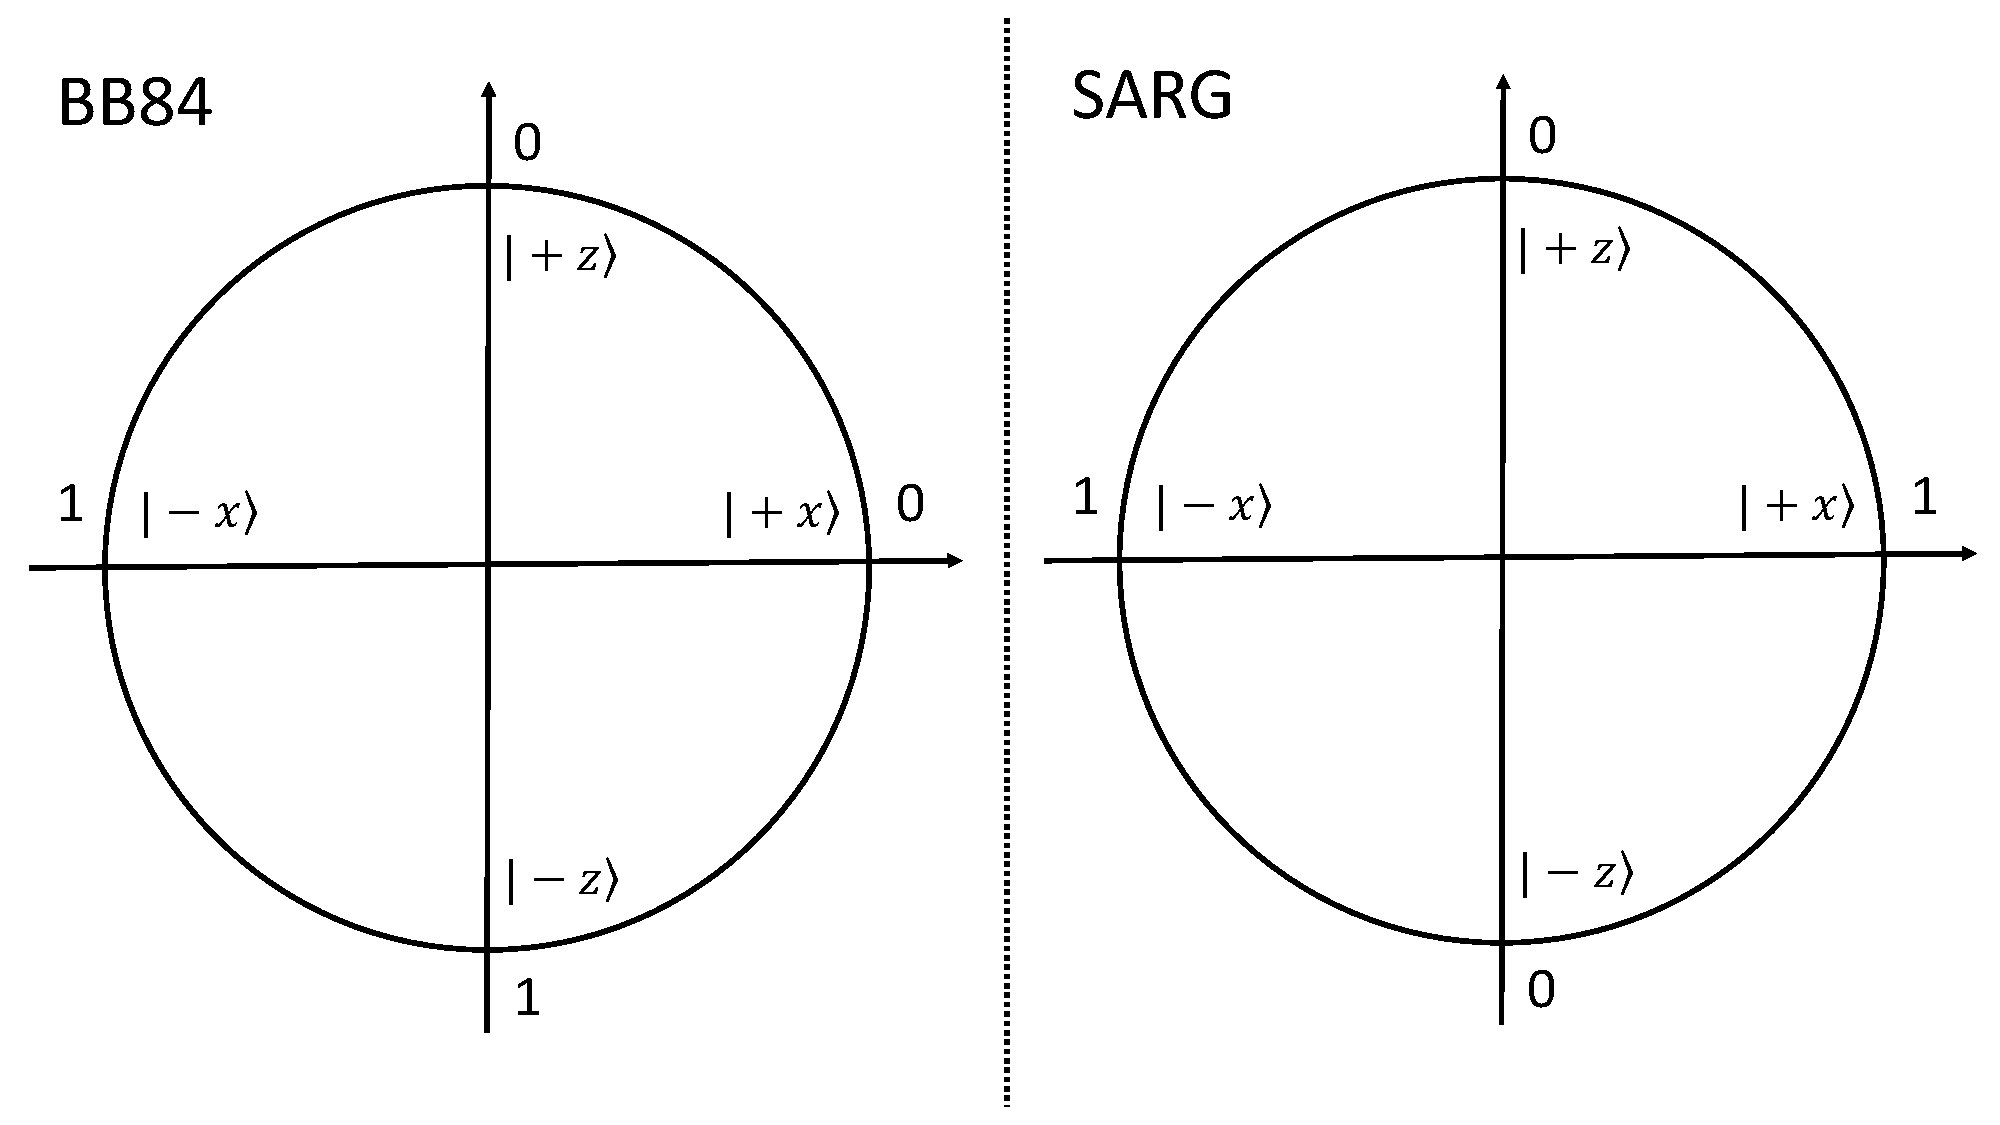
\includegraphics[width=12cm]{SARG.pdf}\\
  \caption{\textbf{SARG encoding:} In the SARG protocol, Alice prepares the same states as in BB84, but the encoding is different. Now, the sent bit is encoded in the prepared basis.}\label{SARGfig}
\end{center}
\end{figure}



The main advantage of the protocol appears when implementing it with weak coherent states because of its robustness against PNS attacks. Recall that the leading order of the attack is given by pulses in which Alice prepares two photons, with probability $p(2)$. In these cases, Eve keeps one photon and waits until the reconciliation to measure her particle. However, in SARG, and contrary to what happens in BB84, Eve has to distinguish between non-orthogonal states, $\ket{+x}$ and $\ket{+z}$ in the previous example, so she cannot perfectly distinguish them and she cannot have full information. It is beyond the scope of the present notes, but it can be proven that for the SARG protocol, and actually for any protocol employing the four BB84 states, Eve can apply another type of PNS attack which gives her full information when using the pulses with three photons. This attack therefore works whenever $p(3)\sim\eta_C\mu$, which gives $\mu^2\sim\eta_C$. Or, in other words, the rate for SARG scales as $R_B\sim \eta_C^{3/2}$, an intermediate scaling between the noiseless case and BB84. 

\subsection{Decoy-state protocols}

The final solution to PNS attacks was provided by Hwang~\cite{decoy} in the form of the so-called decoy-state protocols. In their simplest version, Alice chooses randomly whether to encode her bit in a weak coherent state with intensities $\mu_1$ or $\mu_2$. Experimentally, this is not particularly difficult, all what Alice needs to do is to modulate the light intensity. She sends the state to Bob who measures it as expected in a BB84 implementation. At the end of the protocol, Alice also announces the amplitude she actually used in the encoding, so that Bob can estimate the rate of received photons in the two cases, $R_B^{(1)}$ and $R_B^{(2)}$. In what follows, we show how the use of two amplitudes allows detecting Eve when she implements the standard PNS attack. This is not a full security proof, but it illustrates the main ideas in the protocol.

In the absence of Eve, when Alice and Bob are connected by a purely lossy fibre, the two rates are $R_B^{(i)}=f\mu_i\eta_C$, for $i=1,2$. So the ration between these two amplitudes is equal to the ratio of the coherent-state amplitudes, $R_B^{(1)} /R_B^{(2)}=\mu_1/\mu_2$. When Eve implements the PNS attacks, the rates obtained are basically given by the two-photon pulses, so one has $R_B^{(i)}\sim p_2^{(i)}\sim\mu_i^2$. Therefore, if Eve applied the attack, Alice and Bob would notice an unexpected ratio between the two rates, which would now scale like the square of the ratio of the intensities and not like the ratio itself. In such case, Alice and Bob stop the insecure communication. Adding more intensities makes Eve's life even harder and it can be proven that the expected rate tends to the ideal one proportional to $\eta_C$. 


\section{Hacking attacks}

All the previous discussion shows that security loopholes appear when moving theoretical protocols to the implementation. However, the existence of PNS attacks could not be a priori discarded, because there was no security proof for a weak-coherent state BB84 implementation and large losses. The attacks in fact proved that such a proof was impossible. And the main merit of decoy-state protocols was that a full security proof for them could be established in an implementation with losses and weak coherent states. This proof seemed to end the discussion.

In 2010, however, several successful hacking attacks were reported on QKD commercial implementations for which, a priori, there was a security proof. Vadim Makarov was one of the most active researchers in these quantum hacking efforts~\cite{Makarov}. In the considered BB84 implementation, the last step on Bob's side consisted of sending the received light pulse into a polarised beamsplitter and detect the output modes, see Fig.~\ref{hackingfig}. The hackers modified the working of the detectors on Bob's side by injecting some light on his devices. With this attack, the detectors were no longer sensitive to single photons, but give a click whenever the received light intensity was above a given threshold, $I_{\text{th}}$. Once Eve has modified the working of the detectors, Eve measures the states produced by Alice in a random basis, say $z$, in a given round. She then prepares a new state equal to her result, say $\ket{+z}$, encoded on a light pulse of intensity $I_{\text{th}}<\mu_E<2I_{\text{th}}$  and sends it to Bob through a lossless channel (equivalently, she encodes her bit on a pulse with intensity equal to $\mu_E/\eta_C$, so that what arrives on Bob's side has the right intensity equal to $\mu_E$). Now, if Bob chooses the same measurement as Eve, the pulse will be deterministically sent to one of the two detectors on Bob's side, keeping its intensity above the threshold, and being then detected with the same result as Eve's preparation. If however Bob chooses a different basis than Eve, the coherent state is divided into two pulses of intensities below the threshold and no detection is produced. Bob announces that the photon was lost during the propagation and these rounds are discarded. In total, half of the rounds are discarded, but for those that are kept and later pass basis reconciliation, Alice, Bob and Eve bases agree. Therefore, Eve's attack provides her will full information and her attack does not interfere with Alice's measurement or Bob's preparation. Of course this attack only works if losses are larger than $1/2$, but this is always the case after, approximately, more than 15 kms of optical fibre. 

\begin{figure}
\begin{center}
  % Requires \usepackage{graphicx}
  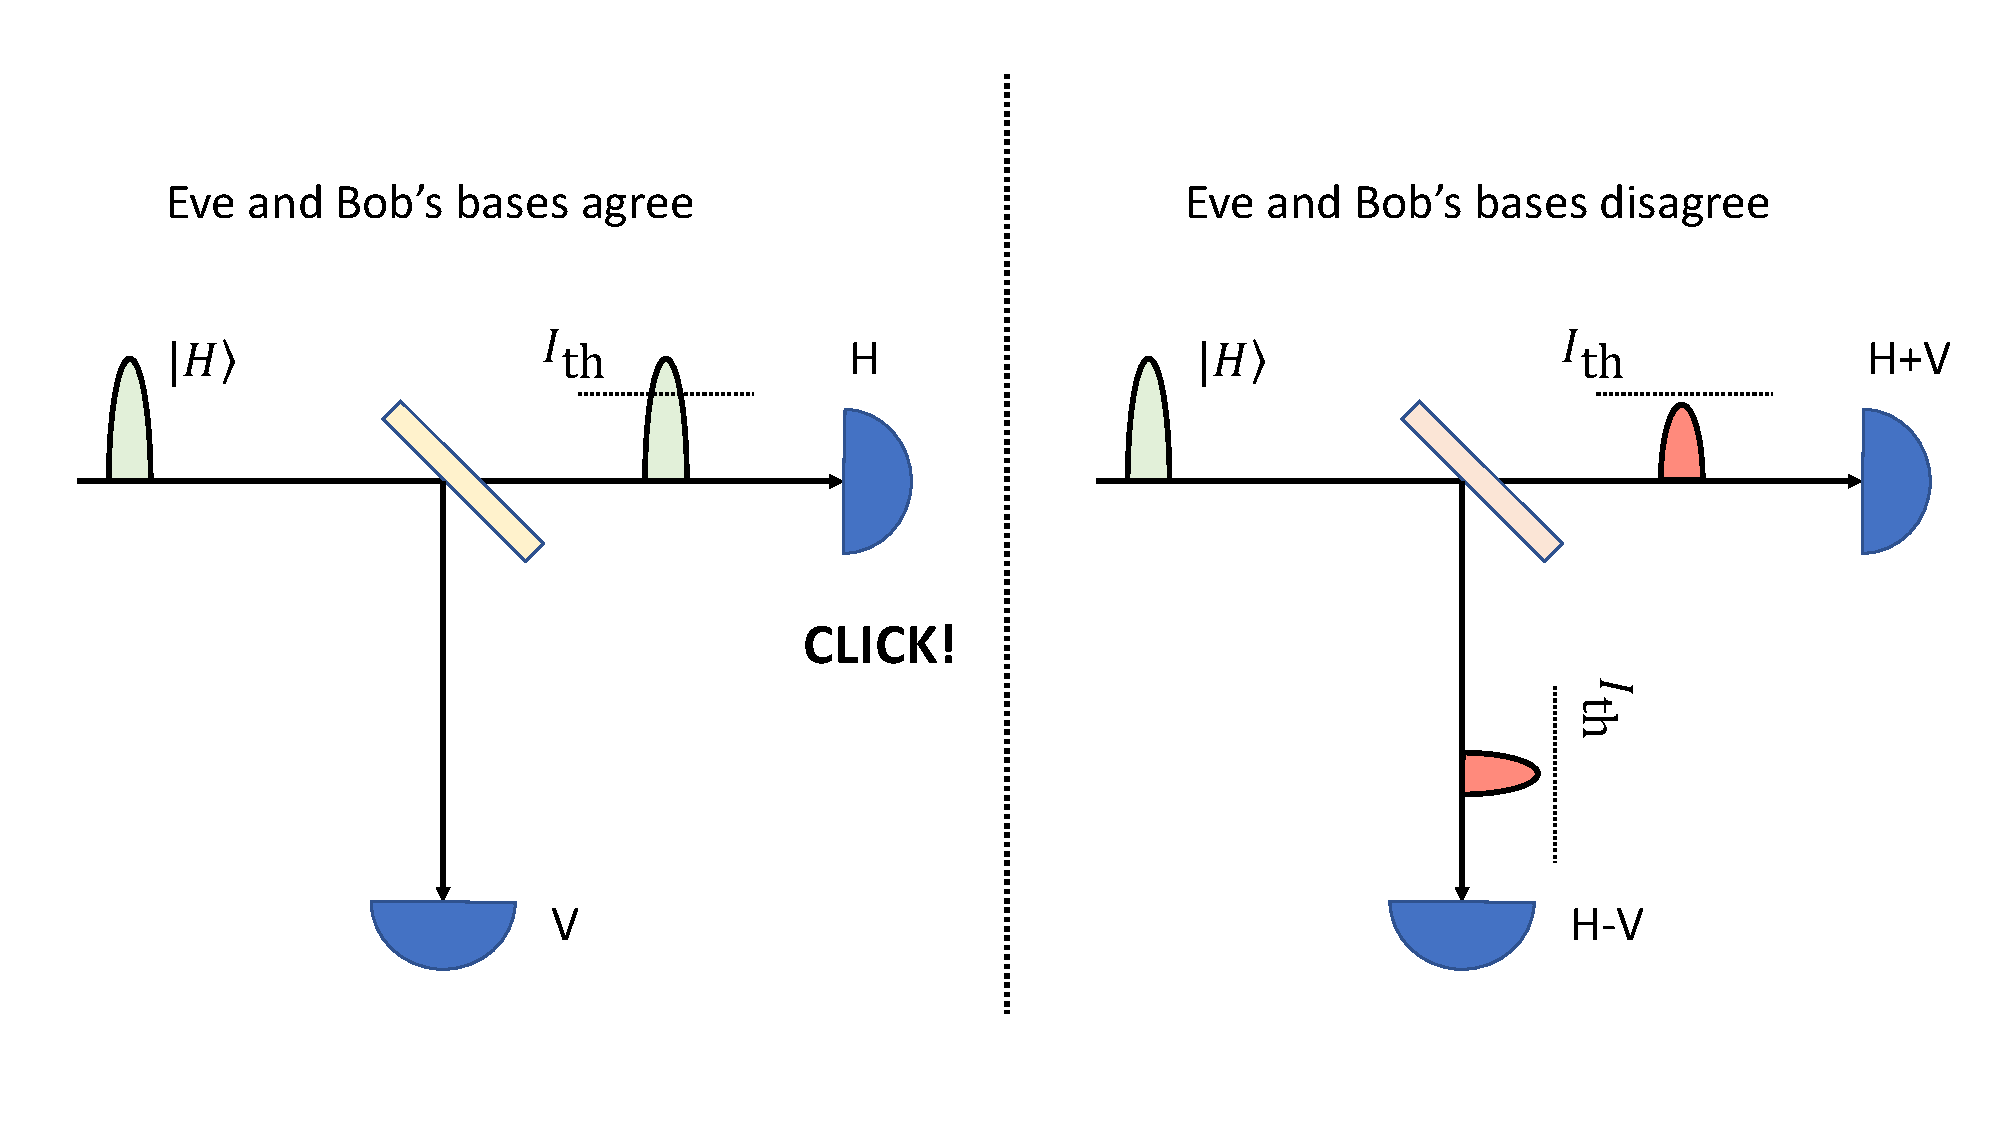
\includegraphics[width=12cm]{Hacking.pdf}\\
  \caption{\textbf{Hacking attack:} Eve injects light on Bob's devices so that they are not sensitive to the incoming photons, but they give a result whenever the incoming light intensity is above the threshold $I_{\text{th}}$. In the attack, Eve measures the state sent by Alice and prepares a new coherent state for Bob equal to her measurement result and with intensity $I_{\text{th}}<\mu_E<2I_{\text{th}}$. If Bob and Eve bases agree, all the light pulse is sent to a detector, giving the prepared result. If the bases disagree, the incoming light pulse is divided into two pulses with intensity below the threshold and giving no detection.}\label{hackingfig}
\end{center}
\end{figure}


The hacking attacks were very important because it was understood that  certifying the security of a quantum implementation is subtler than initially thought. Recall that, in principle, there was a mathematical security proof for the hacked protocol. Was this proof wrong? Or were the hackers able to violate a quantum law and then break the protocol? The answer to these questions is negative and what actually happened was that the implementation did not meet the assumptions needed to prove security. There was a mismatch between the theoretical modelling of the experiment and its implementation, which was exploited by the hackers. The security proof was derived under the assumptions of the model, but if the model is not perfectly accurate in describing the experiment, the obtained security proof does not apply to the implementation, which becomes potentially insecure. 

To better understand this point, let us consider again the BB84. In its formulation, Alice and Bob prepare the eigenstates of $\sx$ and $\sz$ and Bob measures these observables. These are all operators acting on qubit space, $\compl^2$. When thinking of an implementation, it is fundamentally impossible to guarantee that any physical system strictly lives in a Hilbert space of dimension two. Therefore, if the assumptions of the protocol are not met, the security proof does not apply. For instance, consider the situation in which  Alice encodes the qubit in a single-photon state with frequency $\omega_0$. However, let us assume that there is a small imperfection on Alice's devices and whenever she encodes in the $x$ basis, she is slightly shifting this frequency to $\omega'_0=\omega_0+\delta\omega$. If Eve notices this imperfection, all what she needs to do to hack the protocol is (i) first measure the frequency of the single-photon state leaving Alice's lab and (ii) measure in the $z$ ($x$) basis if the measured frequency is $\omega_0$ ($\omega_0+\delta\omega$). She then gets all the information and her attack gets unnoticed. Clearly, this attack can be avoided if Alice initially calibrates her device and corrects this shift, but this won't be the case if the sensitivity of Alice's calibration devices is larger than $\delta\omega$, while Eve's devices can discriminate this frequency shift. Note that the previous four states give very good approximations to the four BB84 states, but they are not identical. In fact, they act on a four-dimensional vector space, spanned by $\{\ket{\pm z,\omega_0},\ket{\pm x,\omega'_0}\}$, hence violating the initial assumption used in the security proof that all the states span a two-dimensional space. To strengthen the security Alice and Bob can try to detect and correct all possible errors of this type and enforce that the gap between the model and the implementation is minimal. In fact, after the hacking attack was announced, the QKD providers corrected the detector in such a way that the specific attack of~\cite{Makarov} was no longer possible. However, how to ensure that no attack exploiting devices' imperfections is possible, especially if we take into account that some assumptions in standard QKD protocols, such as the Hilbert space dimension, are untestable?

\section{The device-independent scenario}

The solution to the previous hacking attacks is provided by the so-called device-independent (DI) scenario~\cite{diqkd}. In this approach, quantum devices are seen as black boxes with which the users can interact providing a classical input and getting a classical output. The DI approach is quite general and, in fact, can be applied to any quantum information protocol, but in what follows we focus on QKD. 

As said, in the DI scenario, devices are seen as quantum black boxes processing a classical input to produce a classical output. It is assumed that the input-output process in a given device takes place locally, that is, it is not causally influenced by what happens in the other devices. This can for instance be enforced by synchronising the devices so that these input-output processes define space-like separated events and therefore there is no time for any signal, not even those propagating at the speed of light, to go from one device to another. However, there may be other ways of enforcing this no-communication assumption.  In a QKD context, Alice and Bob have one device each, see Fig.~\ref{difig}. Without loss of generality, we assume that their inputs, labelled by $x$ and $y$, can take $m$ possible values and their outputs, labelled by $a$ and $b$, can take $r$ possible results, that is $x,y=1,\ldots,m$ and $a,b=1,\ldots,r$. Alice and Bob test their devices using different inputs and collecting the statistics they generate. This is encapsulated by the conditional probability distribution $p(ab|xy)$, which gives the probability that Alice and Bob observe result $a$ and $b$, respectively, when using inputs $x$ and $y$. We therefore have a list of $m^2r^2$ real numbers such that $p(ab|xy)\geq 0$ and $\sum_{ab}p(ab|xy)=1$ for all $x$ and $y$. This conditional probability distribution is also dubbed as \emph{correlations}. The goal of a DIQKD protocol is to conclude from these observed correlations, and only from them, that the parties can distill a secret key. If this is the case, there cannot be any mismatch between modelling and implementation. As said, no modelling is made on these devices, apart from the fact that whatever happens inside to produce the output given the input should be compatible with the quantum laws.


\subsection{Physical correlations}

The main reason why DI applications are possible is because it is assumed that the devices are compatible with a physical theory, in our case quantum mechanics, and this enforces some non-trivial constraints on the observed correlations.

The weakest constraints that can be imposed is that the correlations do not allow for any form of communication between Alice and Bob. As said, this is one of the few assumptions of the formalism, which can for instance be enforced by means of space-time considerations. Some correlations are compatible with this assumption if, and only if, the marginal probability distribution seen by one of the parties, say Alice, is independent of the input used by the other, Bob. In fact, if it was not the case, Bob, by choosing his input, could produce a noticeable effect on Alice, that is he could signal to her. These constraints  are known as no-signalling conditions and give rise to the so-called \emph{non-signalling} correlations. They imply that correlations satisfy the linear constraints
\begin{equation}
\label{nscorrelations}
\forall y: p_A(a|x)=\sum_b p(ab|xy), \quad\quad
\forall x: p_B(b|y)=\sum_a p(ab|xy).
\end{equation}
The set of non-signalling correlations, denoted by $\mathcal{NS}$, is convex and it can be proven that for finite $m$ and $r$, it has a finite number of extreme points, which defines what is called a polytope.

\begin{figure}
\begin{center}
  % Requires \usepackage{graphicx}
  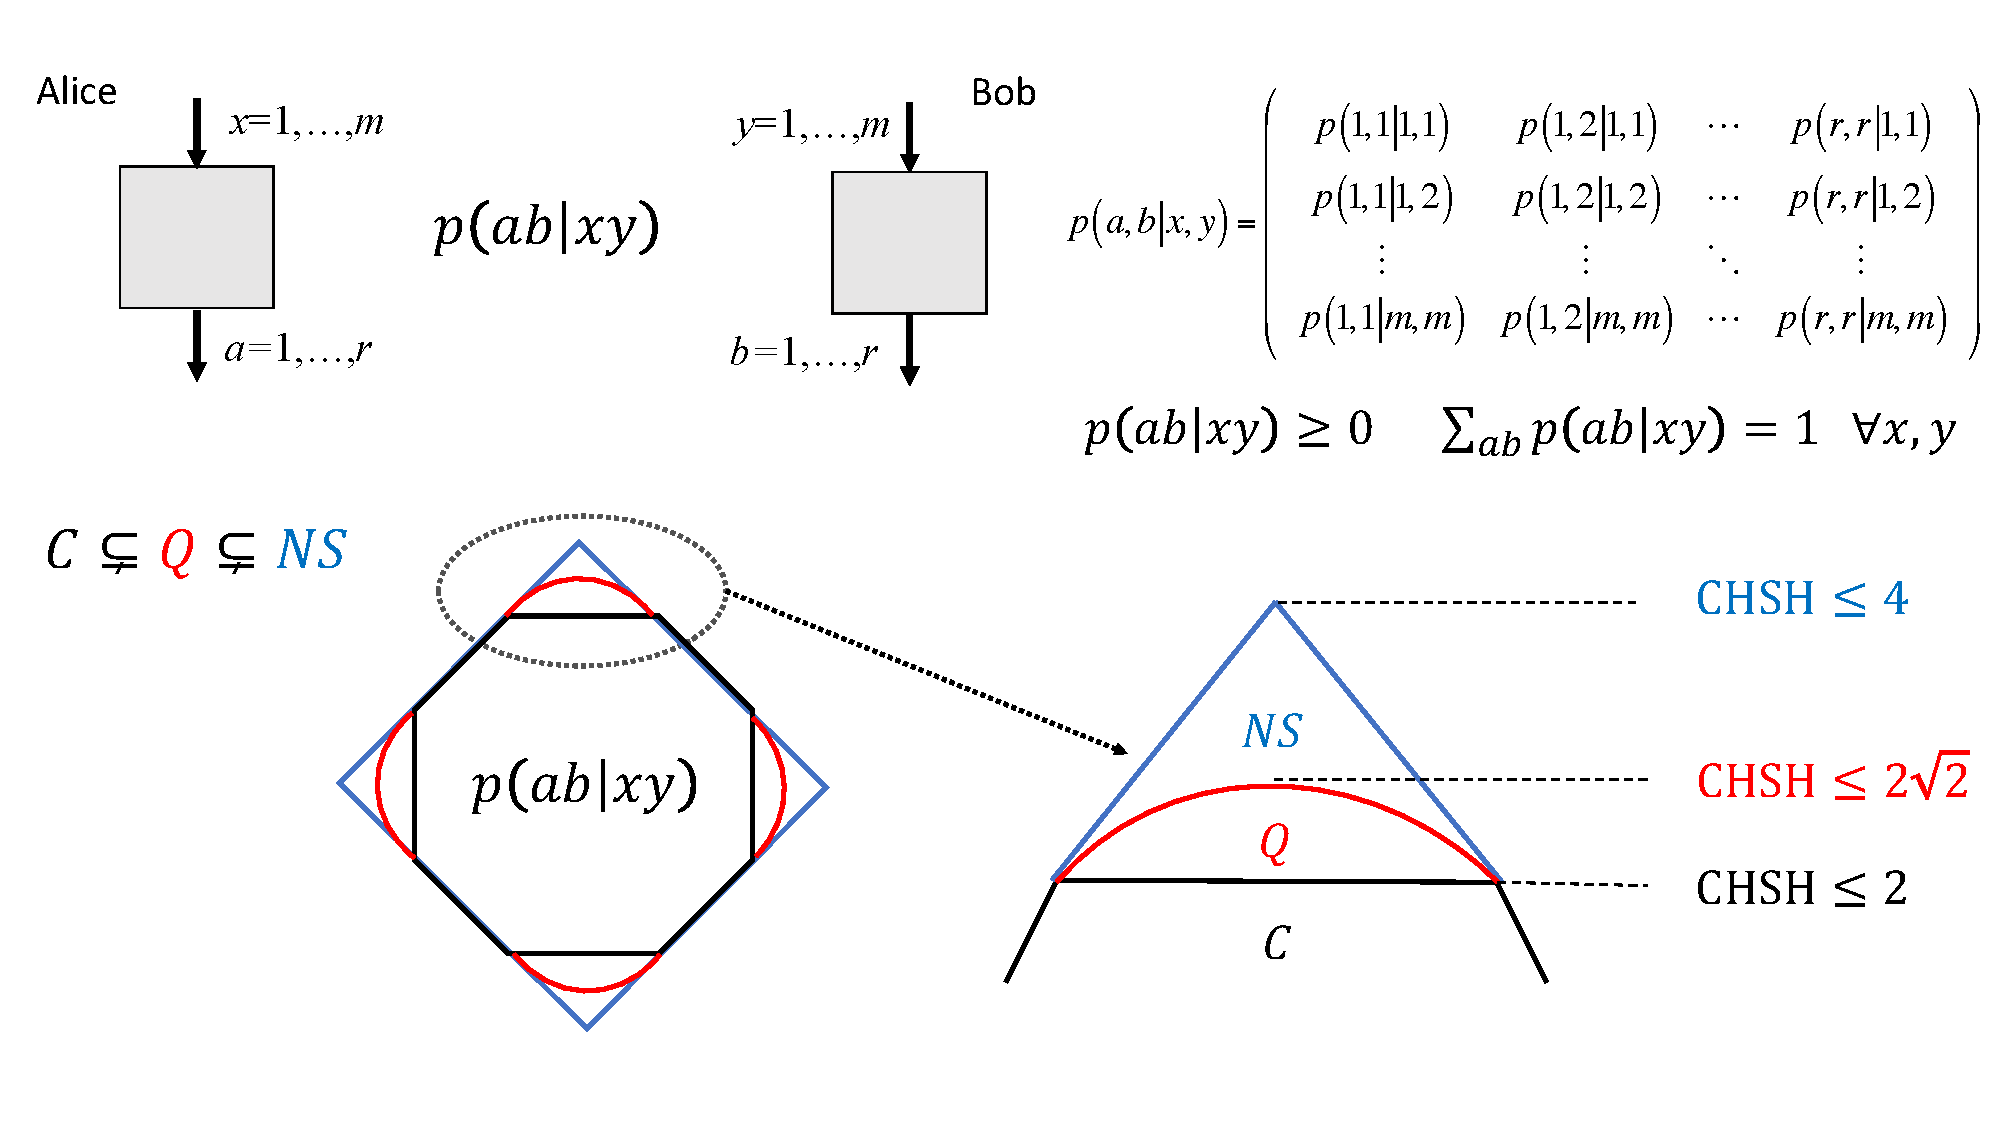
\includegraphics[width=12cm]{Correlations.pdf}\\
  \caption{\textbf{Device-independent scenario:} Alice and Bob model their devices as quantum black boxes producing a classical output given a classical input. The description of the setup is by means of the observed statistics, given by the conditional probability distribution $p(ab|xy)$. There are three main sets of physical correlations: classical, quantum and non-signalling. The first one is strictly includes in the second that, in turn, is also strictly included in the third.}\label{difig}
\end{center}
\end{figure}


Before the advent of quantum theory, the standard way of describing correlations was by means of deterministic classical models. This defines the so-called \emph{classical} correlations, which are those that can be written as
\begin{equation}
p(ab|xy)\sum_\lambda p(\lambda)D_A(a|x\lambda)D_B(b|y\lambda) ,
\end{equation}
where $\lambda$ denotes a correlated classical variables hidden in the devices described by the probability distribution $p(\lambda)$, while $D_A$ and $D_B$ are deterministic functions producing the outputs depending on the inputs and this variable. Classical correlations are nothing but the EPR correlations introduced in~\cite{EPR}. For finite $m$ and $r$, the set of classical correlations $\mathcal C$ is again a polytope, that is, a convex set with a finite number of points.

Finally, the set of interest here is that of quantum correlations. This is defined by those correlations that can be obtained when performing local measurements on a two-party quantum state. We therefore have that some correlations are quantum whenever there exists a state acting on a composite Hilbert space $\mathcal H_A\otimes\mathcal H_B$ and local measurement in each Hilbert space defined by POVMs elements $M_{a|x}$ and $M_{b|y}$, all positive operators such that $\sum_a M_{a|x}=\one_A$ for all $x$ and $\sum_a M_{b|y}=\one_B$ for all $y$, such that
\begin{equation}
\label{qcorrelations}
p(ab|xy)=\tr(\rho_{AB}M_{a|x}\otimes M_{a|x}) .
\end{equation}
Note that we do not impose any specific conditions on the Hilbert spaces used to derive these correlations, they are arbitrary. In particular, the Hilbert space dimension are not specified, that is, the measured systems can be qubits, qutrits, or even have infinite dimension. In fact, the characterisation of quantum correlations, that is, which conditional probability distributions can be expressed as in Eq.~\eqref{qcorrelations}, is very hard, as, intuitively, one needs to explore all possible Hilbert spaces. The set of quantum correlations $\mathcal Q$ is again convex but does not have a finite number of extreme points. 

The relation among these three physical sets is relatively well understood and one has $\mathcal C \subsetneq \mathcal Q \subsetneq \mathcal{NS}$. A pictorial representation of these sets is given in Fig.~\ref{difig}, which reflects the most salient properties of these sets. The first strict inclusion is nothing but a consequence of Bell's theorem, that is the existence of quantum correlations with no classical analogue. In fact, the facets of the classical set define Bell inequalities, hyperplanes defining linear conditions expressed in terms of the observed correlations that are satisfied by all classical correlations (as the set of classical correlations is fully contained on one side of the hyperplane). The second inclusion was proven by Tsirelson and, independently Popescu and Rohrlich~\cite{PRbox}. They derived the so-called Popescu-Rohrlich (PR) box, a conditional probability distribution $p(ab|xy)\in\mathcal{NS}$ that has no quantum realisation. This distribution is obtained for the case of binary inputs and outputs, $m=r=2$. Denoting the values of inputs and outputs by bits, the PR-box is such that $p(ab|xy)=\delta_{a\oplus b=xy}/2$. Here $\oplus$ is the classical XOR, while $xy$ is the AND of these two bits. To understand the notation, we give two examples: $p(a=1,b=1|x=1,y=1)=\delta_{1\oplus 1=AND(1,1)}/2=\delta_{0,1}/2=0$ and $p(a=0,b=0|x=0,y=1)=\delta_{0\oplus 0=AND(0,1)}/2=\delta_{0,0}/2=1/2$. In a more compact way, when $xy=0$ ($xy=1$) the outputs of Alice and Bob are perfectly (anti-) correlated and occur with the same probability. The proof that these correlations are not quantum follows from the fact that they lead to a CHSH value of 4, larger than the maximum allowed by quantum physics, equal to $2\sqrt 2$~\cite{tsirelson}. To see that these correlations produce a CHSH value equal to $4$ is convenient to relabel the outputs as $a,b=\pm 1$ and the inputs as $x,y=1,2$. When the two or one input is equal to 1 (0 in the bit notation used to specify the PR-box), the outputs are perfectly correlated, hence $ab=+1$, so $A_1B_1=A_1B_2=A_2B_1=+1$, while when both inputs are equal to 2 (1 in the bit notation), outputs are perfectly anti-correlated, so one has $A_2B_2=-1$. These values produced the announced non-quantum value of $\text{CHSH}=4$.

After this small parenthesis, devoted to motivate why correlations become non-trivial when combined with a physical theory or even just a physical principle, we present the main ideas to construct device-independent quantum information protocols. Note that in the DI scenario, for Alice and Bob to obtain a result not possible in classical information theory, they should observe correlations that do not have a classical model, that is, correlations that violate a Bell inequality. In fact, Bell inequalities are witnesses of the intrinsically quantum or non-classical origin of these correlations. Since we are going to assume that the devices are quantum, we can focus on correlations in $\mathcal Q$ and discard those correlations in $\mathcal{NS}$ that do not have a quantum realisation.

\subsection{Device-independent quantum key distribution}

We now have most of the ingredients needed to understand the structure of DIQKD protocols. It is important for what follows to understand that in the DI scenario there are two rather different type of players: the users and the provider. The users, Alice and Bob in our case, demand from the provider devices that produce some desired correlations $p(ab|xy)$ that must violate a Bell inequality. These correlations have a specific quantum realisation, but from the user viewpoint this is not relevant, as they want to conclude about their utility to establish a secret key independently of the details of this realisation. The provider, however, does care about the realisation and has to prepare a state and measurements leading to the correlations requested by the user, otherwise the user will not buy the devices.

We stat the discussion with the ideal case and in the simplest scenario of binary inputs and outputs, $a,b,x,y=1,2$. To establish a secret key in the DI setting, Alice and Bob demand devices producing the maximal quantum violation of the CHSH inequality, namely $\text{CHSH}=2\sqrt 2$. However, if one looks at the correlations attaining this value, there are no inputs on Alice and Bob with perfectly correlated outputs. This is why Bob requires a third possible value for his input, $y=3$, whose output is  now perfectly correlated to the output of one of Alice's inputs, say $x=1$. For these combinations of observables, the two results by Alice and Bob have the same probability, but they are identical, that is $\langle A_1\otimes B_3\rangle=1$. Inputs $x=1$ and $y=3$ will be the ones used to establish the secret key and, in fact, they have $I(A:B)=1$. This arrangement defines the so-called CHSH QKD protocol~\cite{diqkd}, where Alice has a binary input to check the CHSH Bell inequality and one of them, $x=1$, is used to establish the secret key, and Bob has an input that takes three values, where two of them, $y=1,2$ are used to compute the CHSH inequality and the third, $y=3$, to establish the key with Alice. To compute Eve's information, Alice and Bob use the fact that there is basically only one way of getting the maximal violations of the CHSH inequality, which is the one in which Alice and Bob share a Bell state~\eqref{bellstate} in which they perform the observables in Fig.~\ref{CHSHfig}. It follows from this result, that we are not going to prove, that the observation of $\text{CHSH}=2\sqrt 2$ implies that that shared state between Alice and Bob is a maximally entangled state of two qubits. Since this state is pure, Eve cannot be correlated, hence her information is zero, $\chi(A:E)=0$. The maximal violation of the CHSH inequality therefore certifies that Alice and Bob can establish a perfect secret key, that is a list of perfectly correlated bits, as $I(A:B)=1$, for which Eve has no information, $\chi(A:E)=0$.

What happens when devices are noisy and, therefore, not attain the maximal CHSH violation? As for standard QKD, one needs to derive a security proof that allows Alice and Bob to bound Eve's information from their observed correlations. Recall however that, when deriving this bound, Alice and Bob should not make any assumptions on their devices, apart from the fact that they produce the observed correlations. Because of continuity, some noise tolerance is to be expected. The main question is whether this tolerance is reasonable and attainable in practical situations. The optimisation problem Alice and Bob have to solve is
\begin{eqnarray}
\label{DIHolevo}
&&\max_{\rho_{AB},\{M_{a|x}\},\{M_{b|y}\}}\chi(A:E)\\
&&\text{such that }\tr(\rho_{AB}M_{a|x}\otimes M_{b|y})=p(ab|xy) .\nonumber
\end{eqnarray}
This optimisation is performed over all possible attacks by Eve, that is all states and measurements in all possible Hilbert spaces compatible with the observed correlations. Note that Eve's Holevo information is a function of the state shared by Alice and Bob and the performed measurements, as the state specifies the purification including Eve, $\ket{\psi}_{ABE}$, to which the measurements are applied to compute $\chi(A:E)$. The optimisation~\eqref{DIHolevo} is in general very hard to solve. One can consider a weaker version of it in which only the observed violation of a Bell inequality, denoted by $\beta$, produced by the correlations between Alice and Bob is used as a constraint, that is, one replaces the constraints on the correlations by $\beta(p(ab|xy)=\beta_{\text{obs}}$. The resulting optimisation is again very hard, but it has been solved for the case of CHSH in~\cite{diqkd}. The obtained solution is equal to 
\begin{equation}
\chi(A:E)=h\left(\frac{1+\sqrt{(\text{CHSH}/2)^2-1}}{2}\right) ,
\end{equation}
where $h(x)=-x\log_2x-(1-x)\log_2(1-x)$ is the binary entropy.  This value allows computing key rates in the case of collective attacks, as for standard QKD protocols. The resulting rates are shows in Fig.~\ref{ratesfig}, together with those obtained for BB84. To make a fair comparison, everything is expressed in terms of the quantum bit error rate (QBER), which also affects the observed Bell inequality violation. The critical QBER, that is, the value for which the Devetak-Winter bound is equal to zero, for the CHSH protocol is $\text{QBER}\approx 7\%$, while it is equal to $\text{QBER}\approx 11\%$ for BB84. The robustness is smaller, as expected because in the DI scenario Eve has more available attacks, but the obtained value of the QBER is realistic and attainable in current experiments.

\begin{figure}
\begin{center}
  % Requires \usepackage{graphicx}
  \includegraphics[width=11cm]{Key Rates.jpg}\\
  \caption{\textbf{Rates for QKD protocols:} Comparison of the Devetak-Winter bounds on the key rate obtained for the standard BB84 protocol, and the DIQKD protocol based on the CHSH Bell inequality, as a function of the QBER. The bound becomes zero for $\text{QBER}\approx 11\%$ and $\text{QBER}\approx 7\%$, respectively.}\label{ratesfig}
\end{center}
\end{figure}


The previous discussion provides the main ideas behind DIQKD protocols and shows how it is possible for Alice and Bob to extract a key without making any assumptions on their devices when exploiting quantum correlations violating a Bell inequality. Recently, a general framework to prove the security of DIQKD protocol has been obtained in~\cite{EAT}. DIQKD provides the strongest form of quantum security. Unfortunately, the realisation of DQIKD protocols is extremely challenging. As we have seen, in practise, Alice and Bob are connected by a lossy channel and Bell violations are very fragile against losses. This explains why, so far, there exist no commercial devices implementing DIQKD protocols and, in fact, only lab demonstrations have recently been achieved~\cite{diexp}. Despite this progress, it remains as a challenging open problem to design ways of observing a Bell inequality violation between distant parties, which in turn can be exploited for secure DIQKD. 


\section{Long-distance Quantum Communication}

In the last part of the notes, we focus on the problem of long-distance quantum communication or, more generally, how to reliably send quantum information through a noisy channel. The scenario is quite similar to what discussed until now, with Alice and Bob in distant locations connected by a quantum channel. However, the goal is now to send quantum information, not to distribute a secret key. Therefore, we do not need to include Eve in the study. 

In the considered scenario, it is assumed that Alice and Bob can perform any type of quantum operations locally and can communicate classical information without any errors. This set of operations is called LOCC, for Local Operations and Classical Communication. The users can exchange quantum states, but only through a noisy channel described by a completely-positive trace-preserving (CPTP) map, $\Lambda$. The goal is to characterise the maximum amount of qubits that can be reliably sent from Alice to Bob as a function of the number of uses of the channel. A formal definition will be provided below.

\subsection{Classical Communication}

The problem of sending information in a reliable way through a noisy channel has a long history in classical information theory. There, a classical channel is described by a stochastic map $P(Y|X)$, describing how an input random variable $X$ is transformed into an output variable $Y$. The standard way of correcting channel errors is through \emph{error correction}. 

As an example, consider the simple binary symmetric channel $P_\epsilon$ that flips a bit with probability $\epsilon$, that is, $P_\epsilon(Y=0|X=0)=P_\epsilon(Y=1|X=1)=1-\epsilon$ and $P_\epsilon(Y=0|X=1)=P_\epsilon(Y=1|X=0)=\epsilon$, which defines the error probability. Without losing generality, the error probability satisfies $\epsilon<1/2$. A very simple error correcting code exploits repetition: to transmit a bit $X$ to Bob, Alice sends its value three times through the channel, $X_1=X_2=X_3=X$. To define the value of his bit, Bob uses the majority of the received symbols, $Y=\text{maj}(Y_1,Y_2,Y_3)$. Clearly, the new error probability is $\epsilon'=3(1-\epsilon)\epsilon^2+\epsilon^3$, which is always smaller than $\epsilon$ when $\epsilon<1/2$.

This example provides the main ideas of error correction. In general, Alice encodes $m$-bit strings $\vec X=(X_1,\ldots,X_m)$, called logical bits, into $2^m$ sequences of $n$ physical bits, $\vec X'=(X'_1,\ldots,X'_n)$, the so-called codewords, through an $m\rightarrow n$ bit encoding map $\mathcal E$. In the previous example, Alice was encoding $m=1$ bits into 2 codewords of $n=3$ bits, namely $000$ and $111$.  On reception, the received message is the one resulting from applying the given channel $P(Y|X)$ to each of the symbols in $\vec X'$. Now, Bob decodes the information by mapping the received $n$-bit string $\vec Y'=(Y'_1,\ldots,Y'_n)$ into an $m$-bit string $\vec Y=(Y_1,\ldots,Y_m)$ through an $n\rightarrow m$ decoding map $\mathcal D$. The error probability for the full protocol is $P(\vec Y\neq\vec X)=\epsilon$ (note that $\epsilon$ now denotes the error probability after error correction). The goal of error correction is, for a given tolerable error $\epsilon$ and $n$ uses of the channel, to maximise the amount of sent bits $m$ over all the possible encoding and decoding maps. We denote this optimum by $m^*(n,\epsilon)$. Now, to understand the ultimate limit for reliable transmission, one should consider the asymptotic rate when the users have access to unlimited uses of the channel and the protocol attains vanishing error probability. This defined the (classical) capacity of the channel, 
\begin{equation}
\label{capacity}
C=\lim_{\epsilon\rightarrow 0} \lim_{n\rightarrow \infty}\frac{m^*(n,\epsilon)}{n} .
\end{equation}

Remarkably, the value of the previous limit is known. Shannon indeed proved that the channel capacity $C$ is given by
\begin{equation}
\label{shannoncapacity}
C=\max_{P(X)} I(X:Y) ,
\end{equation}
where $I(X:Y)$ is the mutual information of the joint distribution $P(X,Y)=P(X)P(Y|X)$, where the first term $P(X)$ is the one to be optimised, while the second $P(Y|X)$ is given by the channel. This result is impressive, as shows how a difficult limit involving $n$ uses of the channel can be computed by solving an optimisation problem involving a single use. This type of formulas, which give the asymptotic performance of an object, in this case a channel, in a given task, reliable communication, only in terms of a single copy of the object are called single-letter formulas. This does not mean that the channel capacity can be attained by a single use of the channel, but that for its computation we only need to consider a single copy of it. In a practical situation, where one has access to a finite number $n$ of uses the channel, one should design an error correction code involving codewords of finite length $n$ that gets as close as possible to the rate $C$. Another consequence of the previous result is that any channel in which the information sent by Alice is not totally erased, that is, any channel where $Y$ is not independent from $X$, $P(Y|X)\neq P(Y)$, can be used for communication. This follows from the fact that $I(X:Y)=0$ if, and only if $P(X,Y)=P(X)P(Y)$.

\subsection{Quantum error correction}

Adapting error correction to the quantum realm is not easy. Error correction somehow builds on redundancy, the repetition of the message, and we know that quantum information cannot be cloned. Also, at decoding, Bob should perform a measurement to read the received state and then decide about how to decode. But quantum measurements perturb the state of the system, hence it seems that the decoding procedure will also introduce errors. In fact, in the early days of quantum information theory, prominent researchers cast doubts on the possibility of quantum error correction~\cite{haroche}.

As first shown by Shor and Steane in~\cite{errcorr}, quantum error
correction is possible. This breakthrough was based on a clever
translation of the known classical techniques to the quantum
formalism, where again $m$ logical qubits are encoded into codewords made of $n$
physical qubits ($(m=1,n=7)$ for Steane's and $(m=1,n=9)$ for Shor's scheme). Now, with this knowledge, we can rephrase the previous discussion on error correction in quantum terms. Given a channel described by a CPTP map $\Lambda$, Alice encodes an $m$-qubit message into $n$ physical qubits through an $n\rightarrow m$ isometry $\mathcal E$ mapping any state $\ket\psi\in\compl^{\otimes m}$ to $\ket{\psi'}=\mathcal E \ket{\psi}\in\compl^{\otimes n}$. These $n$ qubits are now sent through the noisy channel, so Bob receives the $n$-qubit mixed state $\rho'=\Lambda^{\otimes N}(\proj{\psi'})$. Bob applies the decoding map $\mathcal D$ to this state, getting $\rho=\mathcal D(\rho')$. The goal of the protocol is that this state is $\epsilon$-close to the encoded state $\ket\psi$, that is, $\bra\psi\rho\ket\psi\geq 1-\epsilon$ for a given error threshold $\epsilon$.



It is far from the scope of these
notes to give a detailed explanation of quantum error correction.
However, we provide in what follows a simple scheme that shows how to improve the error rate of
the noisy channel 
\begin{equation}
\Lambda_x(\rho)=(1-p_x)\rho+p_x\sx\rho\sx ,
\end{equation}
that is, a channel in which with probability $1-p_x$ the state does not change, while a bit flip $\sx$ is performed with probability $p_x$. It is a rather academic channel, but it is enough to illustrate how
quantum error correcting techniques work.

The goal is to present an encoding and decoding process that does the analogue of the simple classical $1\rightarrow 3$ repetition code described above.
A representation of this scheme is shown in Fig.~\ref{errc}. The initial qubit to be transmitted is in an arbitrary state $\ket\psi=\alpha\ket 0 +\beta\ket 1$. Alice encodes it into a 3-qubit state by the isometry in which she adds two new qubits in state $\ket 0$ and performs two CNOT operations as shown in Fig.~\ref{errc}. The resulting state is $\ket{\psi'}=\alpha\ket{000}+\beta\ket{111}$. Note that the $1\rightarrow 3$ repetition is somehow achieved keeping the coherences in the state. This state is now sent through the channel, so the state received by Bob is $\rho'=\Lambda_x^{\otimes 3}(\proj{\psi'})$. It is easy to see that this state can be written as
\begin{equation}
\rho'=(1-p_x)^3\rho'_0+3(1-p_x)^2p_x\rho'_1+3(1-p_x)p_x^2\rho'_2+p_x^3\rho'_3 ,
\end{equation}
where
\begin{eqnarray}
&&\rho'_0=\proj{\psi'}\nonumber\\
&&\rho'_1=\frac{1}{3}\left(\sx\otimes\one\otimes\one\proj{\psi'}\sx\otimes\one\otimes\one+\one\otimes\sx\otimes\one\proj{\psi'}\one\otimes\sx\otimes\one\right.\nonumber\\
&\quad&\left.\quad\quad+\one\otimes\one\otimes\sx \proj{\psi'} \one\otimes\one\otimes\sx\right) \nonumber\\
&&\rho'_2= \frac{1}{3}\left(\sx\otimes\sx\otimes\one \proj{\psi'} \sx\otimes\sx\otimes\one + \sx\otimes\one\otimes\sx \proj{\psi'} \sx\otimes\one\otimes\sx\right.\nonumber\\
&\quad&\left.\quad\quad+\one\otimes\sx\otimes\sx \proj{\psi'} \one\otimes\sx\otimes\sx\right) \nonumber\\
&&\rho'_3= \sx\otimes\sx\otimes\sx \proj{\psi'} \sx\otimes\sx\otimes\sx ,
\end{eqnarray}
that is, all the different terms where zero, one, two or three errors take place. Note the analogies with the classical case. Now, the goal is to design a map correcting all instances with zero and one error, that is $\mathcal D(\rho'_0)=\mathcal D(\rho'_1)=\proj\psi$. The circuit in Fig.~\ref{errc} achieves this, as we are going to shown for each of the pure states appearing in these mixed states.

\begin{figure}
\begin{center}
  % Requires \usepackage{graphicx}
  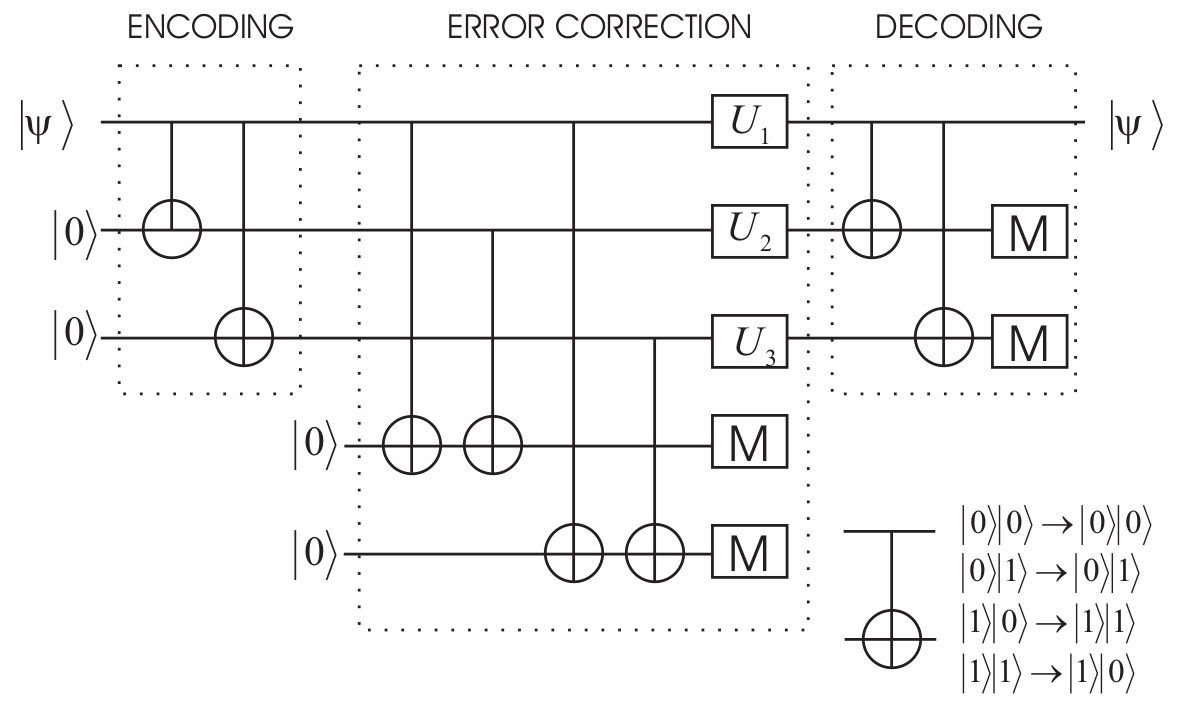
\includegraphics[width=10cm]{errcorr}\\
  \caption{\textbf{Quantum error correction:} The figure shows a simple example of encoding and decoding operations correcting at most one bit flip.
  The measurements on the fourth and fifth qubit inform Bob about which unitary operations $U_1$, $U_2$ and $U_3$ to implement to fix the error in one (or none) of the three physical qubits encoding the logical qubit
  in state $\ket{\psi}$.}\label{errc}
  \end{center}
\end{figure}


\begin{itemize}
    \item No errors: Bob receives the encoded state
    $\ket{\psi'}=\alpha\ket{000}+\beta\ket{111}$. One can see that the state after adding the extra two qubits and implementing the CNOTs in the error correction part is $(\alpha\ket{000}+\beta\ket{111})\ket{00}$. The measurements of the last two qubits give $00$. Basically, this circuit leaves the state in the first three qubits unchanged, as they are controlling the result of the CNOT gates, while the two bits obtained in the measurement, see Fig.~\ref{errc}, extract the information about the error: they inform about whether qubit 1 and 2 are identical, or whether qubit 1 and qubit 3 are equal. In the present case, since the result is 00, Bob deduces that the three qubits are equal. This is compatible with no error, or three errors, but the first one is more likely, so he does nothing $U_1=U_2=U_3=\one$. The state entering into the final decoding part is again  $\ket{\psi'}=\alpha\ket{000}+\beta\ket{111}$, which is mapped into $\ket{\psi}=\alpha\ket{0}+\beta\ket{1}$ by the two final CNOT operations and measurements. In fact, these two last measurements are not really needed.
    \item Error on the first qubit: Bob receives the state
    $\alpha\ket{100}+\beta\ket{011}$. After the series of CNOT's
    gates, one has $(\alpha\ket{100}+\beta\ket{011})\ket{11}$. The two measurements on the last two qubits give 11. This is informing Bob that qubit 1 is different from 2, and also from 3. If there was only one error, Bob knows he has to correct the first qubit, so
    applies $U_1=\sigma_x$ and $U_2=U_3=\one$. The resulting state is again $\ket{\psi'}=\alpha\ket{000}+\beta\ket{111}$, so the final decoding part
    provides the initial state.
    \item Error on the second qubit: Bob receives the state
    $\alpha\ket{010}+\beta\ket{101}$. The reasoning proceeds as
    above, but now the state before the first measurement is $(\alpha\ket{010}+\beta\ket{101})\ket{10}$. The measurements give 10 and inform Bob that the second qubit was different from the other two, hence he corrects it, $U_2=\sigma_x$ and $U_1=U_3=\one$. The last part is identical as in the previous step
    \item Error on the third qubit: Bob receives the state
    $\alpha\ket{001}+\beta\ket{110}$. Same as above, but now the
    measurements on the fourth and fifth qubit give 01, so Bob infers that the third qubit is wrong and applies $U_3=\sigma_x$ and
    $U_1=U_2=\one$.
\end{itemize}

This simple scheme illustrates how quantum error correcting work: (i) Alice encodes the
$m$ initial logical qubit into quantum codewords made of $n$ physical
qubits; (ii) after the propagation through the channel, some of the
qubits are measured, providing Bob information about the errors
occurred in the channel; (iii) the error is corrected and the
original quantum state decoded. A real quantum error correcting
method should correct not only bit flips, $\sigma_x$, but also
phase flips, $\sigma_z$, and any arbitrary combination of them. As
said, such schemes do exist and constitute a basic primitive on
any implementation of quantum information processing, especially for quantum computation purposes.

We now have all the ingredients to define the quantum capacity $\text{QC}$ of a quantum channel $\Lambda$. First of all, for $n$ uses of the channel, we define $m^*(n,\epsilon)$ as the maximum number of qubits that can be transmitted with error $\epsilon$. This means that there exist encoding and decoding maps, $\mathcal E$ and $\mathcal D$, such that for all $\ket\psi\in\compl^{\otimes m}$, one has $\bra\psi\rho\ket\psi\geq 1-\epsilon$, where $\rho=(\mathcal D\circ\Lambda^{\otimes n}\circ\mathcal E)(\proj\psi)$. Then, the quantum capacity of the channel is defined as in Eq.\eqref{capacity}, with this new definition of $m^*(n,\epsilon)$.

While the formal definition of capacities for classical and quantum channels look almost identical, there are several important differences. First of all, and contrary to what happens in the classical case, there exist channels with zero quantum capacity, $\text{QC}=0$, although the state received by Bob depends on Alice's preparation. The easiest examples of such channels are given by the so-called two-shareable channels. These are channels $\Lambda$, say from $A\rightarrow B$, such that there exists another channel $\tilde\Lambda$ from $A\rightarrow B_1B_2$ with the property that, for all input states $\rho$, one has $\tr_1(\tilde\Lambda(\rho))=\tr_2(\tilde\Lambda(\rho))=\Lambda(\rho)$. In fact, supposed that the original channel was such that $\text{QC}>0$. This would mean that there exist encoding and decoding operations such that  $\bra\psi(\mathcal D\circ\Lambda^{\otimes n}\circ\mathcal E)(\proj\psi)\ket\psi\geq 1-\epsilon$. Now, one could then apply the encoding to a state $\ket\psi$, use it as input to $\tilde\Lambda$ and apply the decoding map to the output states $B_1$ and $B_2$, getting two copies of the initial state of arbitrarily good quality, and therefore violating the no-cloning theorem. That is, the cloning theorem implies the existence of non-trivial channels with zero quantum capacity. Note that there are very natural examples of two-shareable channels, possibly the simplest being a lossy channel in which a state is transmitted with probability $1/2$ from $A$ to $B$. It can trivially be shared by a channel in which the state is transmitted either to $B_1$ and $B_2$ with probability $1/2$. Recall that this channel appears in optical fibre communications and, in fact, a transmission below $1/2$ is obtained at relatively short distance. This implies that quantum error correction is of limited use for quantum communication purposes. 

Second, in the quantum case, we do not know whether a single-letter formula for the quantum channel capacity exists and, in fact, it is conceivable that it does not. Third, and this is related to the previous point, the quantum capacity is non-additive~\cite{smithyard}: there exist quantum channels $\Lambda_1$ and $\Lambda_2$ such that (i) $\text{QC}(\Lambda_1)=\text{QC}(\Lambda_2)=0$, but (ii) $\text{QC}(\Lambda_1\otimes\Lambda_2)>0$. In other words, two channels that are useless to send quantum communication, become useful when combined. This astonishing property of quantum information is in fact more common than initially expected, as there are several operational scenarios in which quantum information properties are not additive, the quantum capacity being one of the most famous examples. This non-additivity property is sometimes encapsulated by the funny formula $0+0>0$.




\subsection{Entanglement-based quantum communication}

Quantum error correction represents a solution for solving the
imperfections in the channel. However, if the errors in the
channel are too large, there cannot be any quantum error
correcting code allowing the faithful transmission of quantum
information through the channel. As said, this is in strong contrast to what
happens for classical information: even if the errors in the
channel are very large, there is always an encoding and decoding
process allowing a noise-free error transmission. When dealing with quantum channels, quantum
error correction may be impossible even in situation where Bob's
quantum state is correlated to Alice's initial state. Therefore, the problem of long-distance quantum communication should explore other methods and the solution again comes through entanglement.

Before proceeding, note that in a quantum communication scenario, if the parties are initially assisted by a maximally entangled state, say of two qubits Eq.~\eqref{bellstate}, then Alice can perfectly send a qubit to Bob by means of quantum teleportation~\cite{teleportation}. At the end of this protocol, the entanglement is destroyed, so sharing a maximally entangled state is equivalent in this context to use once the identity channel $\Lambda(\rho)=\rho$, that is, a perfect channel with no errors. Let us now see how to make use of this idea.

If Alice and Bob are connected by a channel $\Lambda$, say of one qubit, and Alice is thinking of using teleportation, she can try to establish entanglement with Bob by locally preparing a two-qubit entangled state and then sending half of it through the channel. At the end of this process, Alice and Bob share the state
\begin{equation}
\rho_{AB}=(\one\otimes\Lambda)(\proj{\Phi^+}) .
\end{equation}
Now, suppose that this state can be transformed by LOCC into a maximally entangled state with some probability $p$. This process is called \emph{entanglement distillation}. Then, the resulting maximally entangled state can be used to teleport a qubit reliable from Alice and Bob. If they repeat this process $n$ times, Alice and Bob will deterministically get of the order of $np$ maximally entangled states, and hence will be able to transmit of the order of $np$ qubits.

This procedure works for channels that are two-shareable, where quantum error correction is useless. A simple example is the channel with transmission coefficient $1/2$. In fact, it works for any purely lossy channel of transmission $\eta_C$. When sending half of a maximally entangled state, say encoded in two photons, through it, Alice and Bob end up with the state
\begin{equation}
\rho_{AB}=\eta_C\proj{\Phi^+}+(1-\eta_C)\frac{\one}{2}\otimes\proj\varnothing ,
\end{equation}
where $\ket\varnothing$ is the state associated to the loss of the photon. Now, Bob can now implement the two output measurement described by the Kraus operators
\begin{equation}
A_{\text{ok}}=\proj 0+\proj 1\quad A_{\text{loss}}=\proj\varnothing .
\end{equation}
This is nothing than Bob observing whether the particle, in our example the photon, encoding half of the maximally entangled state has made it through the channel without destroying it. It is an example of the so-called quantum non-demolition measurements, which are challenging but possible.  It is clear than when Bob gets the result $r=\text{ok}$, which happens with probability $\eta_C$, the state between Alice and Bob is projected into $\ket{\Phi^+}$. 
 
 This result shows that quantum information can be transmitted through any purely lossy channel, with a rate that goes at least as $\eta_C$. This is not in contradiction with the previous result using quantum error correction. In fact, the previous expression for the quantum channel capacity was defined in terms of quantum error correction protocols in which information only goes from Alice to Bob. This implies that our previous definition was in fact encapsulating the so-called one-way communication capacity, denoted by $\textbf{QC}^\rightarrow$. In particular, this capacity is zero for two-shareable channels. However, in the previous protocol using entanglement distillation, Bob needs to communicate with Alice to inform her about the result of his measurement, and this message goes in the opposite direction. A more general protocol could in fact involve several rounds of classical communication from Alice to Bob and viceversa. To take into account this possibility, we will define below the two-way quantum capacity $\text{QC}^\leftrightarrow$. 
 
The previous discussion shows that the problem of long-distance quantum communication is intimately connected to the problem of entanglement distillation through the channel. In fact, imagine that the channel would allow the distribution of states that are distillable, that is, that Alice and Bob could establish after $n$ uses of the channel a state that can be transformed into $m$ maximally entangled states of two qubits. Then, these $n$ uses would allow the exchange of $m$ qubits through teleportation. On the other hand, imagine that,  using $n$ times the channel, Alice and Bob could reliable distribute $m$ qubits. Then, Alice could apply this protocol to reliably send the $m$ halves of $m$ maximally entangled states to Bob, hence perfectly distributing entanglement.
It therefore follows that the two-way quantum capacity can be defined as follows. Consider $n$ uses of the channel acting on the $n$ halves of $n$ maximally entangled states, resulting in a state equal to $n$ copies of $\rho_{AB}=(\one\otimes\Lambda)(\proj{\Phi^+})$. Now, define $m^*(n,\epsilon)$ as the maximum number $m$ of maximally entangled states that can be distilled from this state by LOCC with an error $\epsilon$, that is, $^{\otimes m}\bra{\Phi^+}\text{LOCC}(\rho_{AB}^{\otimes n})\ket{\Phi^+}^{\otimes m}\geq 1-\epsilon$. Then, the two-way quantum capacity is defined as in~\eqref{capacity}. For example, it follows from what has been said above that a lossy channel has $\text{QC}^\leftrightarrow>\text{QC}^\rightarrow=0$, proving the advantage of two-way communication strategies.

\subsection{Quantum repeaters}

The use of entanglement distillation enlarges the set of channels that allow reliable quantum communication. Still, this is not the final solution. In fact, there exist states from which one cannot distill maximally entangled states. The simplest example is given by separable states: clearly no entanglement can be distilled from a non-entangled state. Moving to channels, there exist channels for which any output state is separable. These channels are called \emph{entanglement breaking}, for obvious reasons. It is known that a channel $\Lambda$ is entanglement breaking if, and only if, the state obtained when applying the channel to half of a maximally entangled state is separable. A simple example of such channels is given by the depolarising channel, Eq.~\eqref{depchannel}, with $0\leq p\leq 1/3$. There are even channels that allow the distribution of entanglement, but the obtained entangled states cannot be distilled into maximally entangled states, these states being known as \emph{bound entangled}~\cite{horodecki}. Entanglement breaking channels, or channels that at most distribute bound entanglement have $\text{QC}^\leftrightarrow=0$. Beyond these more academic considerations, even for the purely lossy channel, and despite the fact that channel has in principle a positive quantum capacity for all losses, the quantum communication rate scales with the transmission of the channel, hence decreasing exponentially with the distance between Alice and Bob. In a realistic implementation, quantum communication becomes impractical after, say, a few hundreds of kms.

In fact, already in classical information theory, and despite the fact that all non-trivial channels have strictly positive quantum capacity, direct transmission becomes at some point useless. The solution consists of dividing the long lossy channel into segments in which to place nodes, or repeaters, that read the information, correct it and prepare a new perfect copy for the next node. If one literally followed this idea, one would need to place repeaters as soon as the channel does not allow quantum error correction, which would imply that repeaters would be needed after very short distances. The solution to that is to combine the idea of repeater with entanglement, leading to the concept of \emph{quantum repeater}~\cite{qrep}. The idea exploits many of the tools explained above, plus the protocol of entanglement swapping. Entanglement swapping considers the situation in which the teleportation protocol is applied to half of a maximally entangled state. This protocol is already discussed in the original teleportation paper~\cite{teleportation}, and expanded in~\cite{entswap}. Imagine the situation in which three parties share two maximally entangled states as follows: Alice shares a maximally entangled state $\ket{\Phi^+}_{AB_1}$ with Bob, who in turns shares another maximally entangled state $\ket{\Phi^+}_{B_2C}$ with Charlie. Now, if Bob teleports particle $B_1$ to Charlie using this second state, the entanglement is swapped and now Alice and Charlie share a state $\ket{\Phi^+}_{AC}$, while any entanglement with Bob is destroyed. Bob's measurement maps the entanglement he has with Alice and Charlie to direct entanglement between them.

The intuitive idea of a quantum repeater is as follows, see also Fig.~\ref{qrepfig}. Consider two distant parties connected by a very noisy channel for which direct quantum communication is impractical, or even impossible. Several intermediate stations, the so-called repeaters, are placed through the channel, so that the effective channel between any consecutive repeaters has a much better quality. Now, entangled states are distributed through the different nodes. Since the channels have a better quality, the resulting less noisy entangled states can now be distilled into maximally entangled states connecting all the nodes in the channel. The parties then perform entanglement swapping so that all the entangled pairs are now shared between the two end nodes, Alice and Bob. Finally, Alice and Bob use these pairs to reliably exchange quantum communication through teleportation. The protocol while theoretically appealing, is however very challenging, as the nodes need to perform operations on several qubits and store them in memories without decoherence while the protocol is executed. No demonstration of any repeater configuration, not even with one single repeater and in a lab environment, has been achieved yet, although several groups worldwide are intensively working on developing all the ingredients needed for that.

\begin{figure}
\begin{center}
  % Requires \usepackage{graphicx}
  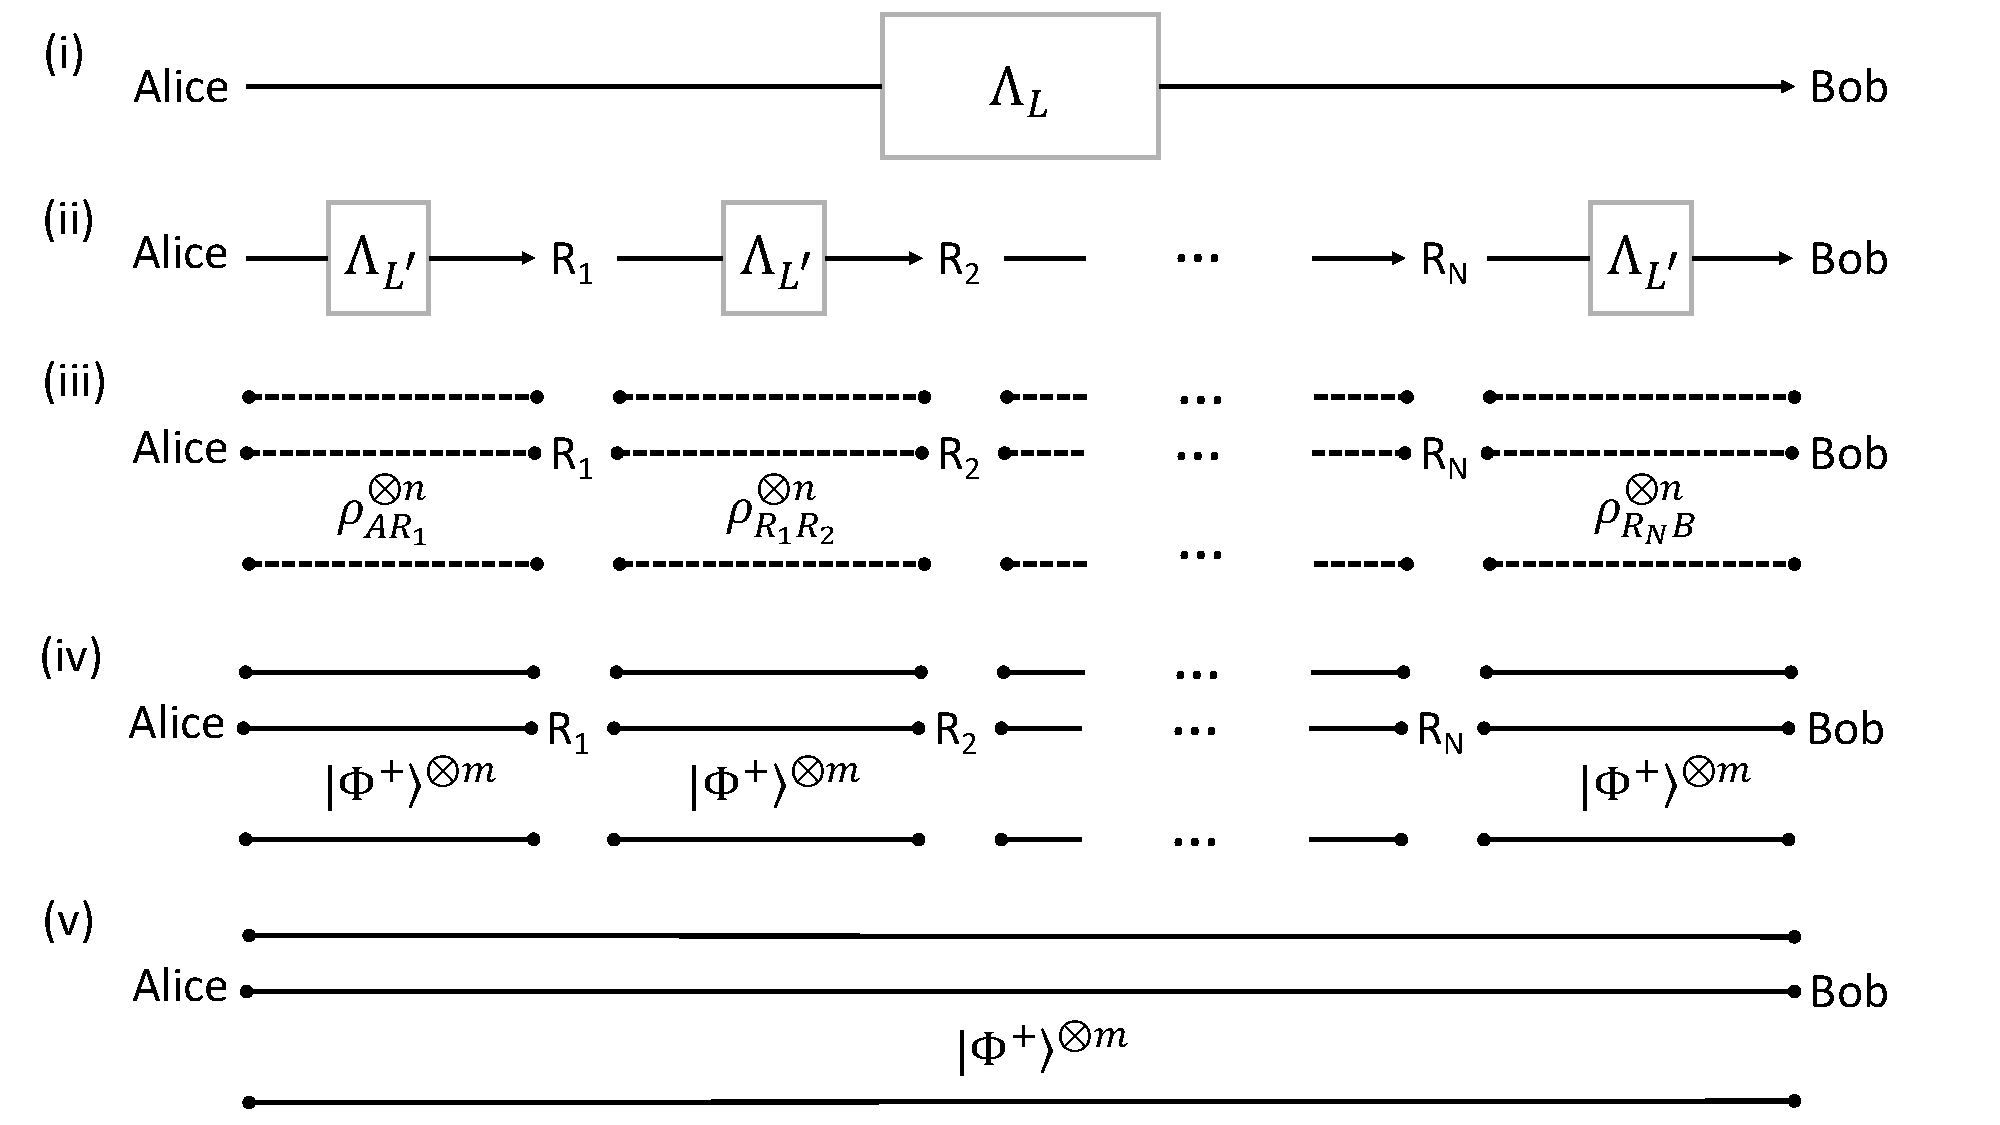
\includegraphics[width=13cm]{QRepeater.pdf}\\
  \caption{\textbf{Quantum repeaters:} (i) Alice and Bob are connected by a very noisy channel $\Lambda_L$, where quantum communication is impractical or even impossible. (ii) Intermediate repeater stations are added, so that the resulting channel connecting different nodes, $\Lambda_{L'}$ has a much better quality and allow for the distribution of distillable entangled states. (iii) The parties use $n$ times the channel to distribute entanglement, resulting in $n$ copies of a mixed entangled state. (iv) These mixed states are distilled into $m$ maximally entangled states by LOCC. (v) The entanglement is mapped to the end nodes by means of entanglement swapping, so that reliable quantum communication is now possible through quantum teleportation.}\label{qrepfig}
  \end{center}
\end{figure}



Putting all these ideas together, we arrive at the concept of the \emph{quantum internet}~\cite{kimble}, where different nodes will be able to have quantum computers able to perform any quantum operations on their states and store them in quantum memories and exchange quantum bits though entanglement and teleportation. This is the ultimate goal of quantum communication.










\begin{thebibliography}{99}

\bibitem{NC}
M. A. Nielsen and I. L. Chuang, {\sl Quantum Computation and Quantum Information},
Cambridge University Press.

\bibitem{revcomp}
C. H. Bennett, IBM J. Res. Develop. {\bf 17}, 525 (1973); IBM J.
Res. Dev. {\bf 32}, 16 (1988).

\bibitem{universal}
A. Barenco, C. H. Bennett, R. Cleve, D. P. DiVincenzo, N.
Margolus, P. Shor, T. Sleator, J. A. Smolin and H. Weinfurter
Phys. Rev. A {\bf 52}, 3457 (1995).

\bibitem{twoqubit}
M. J. Bremner, C. M. Dawson, J. L. Dodd, A. Gilchrist, A. W.
Harrow, D. Mortimer, M. A. Nielsen, T. J. Osborne, Phys. Rev.
Lett. {\bf 89}, 247902 (2002).

\bibitem{BMPRV}
P. O. Boykin, T. Mor, M. Pulver, V. Roychowdhury and F. Vatan,
quant-ph/9906054.

\bibitem{noclon}
W. K. Wootters and W. H. Zurek, Nature {\bf 299}, 802 (1982).

\bibitem{EPR}
A. Einstein, B. Podolsky and N. Rosen, Phys. Rev. {\bf 47}, 777
(1935).

\bibitem{Bell}
J. S. Bell, Physics {\bf 1}, 195 (1964).

\bibitem{Aspect}
A. Aspect, P. Grangier and G. Roger, Phys. Rev. Lett. {\bf 47},
460 (1981).

\bibitem{exp}
W. Tittel {\sl et al.}, {\sl ibid} {\bf 81}, 3563 (1998); G.
Weihs {\sl et al.}, {\sl ibid} {\bf 81}, 5039 (1998); M. Rowe {\sl
et al.}, Nature {\bf 409}, 791 (2001).

\bibitem{hanson}
B. Hensen {\sl et al.}, Nature \textbf{526}, 682 (2015).

\bibitem{nist}
M. Giustina {\sl et al.}, Phys. Rev. Lett. \textbf{115}, 250401 (2015).

\bibitem{vienna}
L.~K. Shalm {\sl et al.}, Phys. Rev. Lett. \textbf{115}, 250402 (2015).

\bibitem{CHSH}
J. F. Clauser, M. A. Horne, A. Shimony and R. A. Holt, Phys. Rev. Lett. \textbf{23}, 880 (1969).

\bibitem{tsirelson}
B. S. Tsirelson, Lett. Math. Phys. \textbf{4}, 93 (1980)

\bibitem{BB84} C.H. Bennett and G. Brassard,
Proceedings IEEE Int. Conf. on Computers, Systems and Signal
Processing, Bangalore, India (IEEE, New York, 1984), pp. 175-179.

\bibitem{B92}
C. H. Bennett, Phys. Rev. Lett. \textbf{68}, 3121 (1992).

\bibitem{6state}
D. Bru\ss{}, Phys.Rev.Lett. \textbf{81}, 3018  (1998).

\bibitem{vaidman}
L. Goldenberg and L. Vaidman, Phys. Rev. Lett. \textbf{75}, 1239 (1995).

\bibitem{Ekert}
A. Ekert, Phys. Rev. Lett. \textbf{67}, 661 (1991).

\bibitem{BBM}
C.~H. Bennett, G. Brassard and N.~D. Mermin, Phys. Rev. Lett. \textbf{68}, 557 (1992).

\bibitem{renner}
R. Renner, arXiv:quant-ph/0512258.

\bibitem{dwrate}
I. Devetak and A. Winter, Proc. R. Soc. Lond. A  \textbf{461}, 207 (2005).

\bibitem{Holevo}
A. S. Holevo, Probl. Inf. Trans. {\bf 9}, no. 3, 177 (1973).

\bibitem{PNS}z
G. Brassard, N. L\"utkenhaus, T. Mor and B. C. Sanders, Phys. Rev. Lett. 85, \textbf{1330} (2000).

\bibitem{SARG}
V. Scarani, A. Ac\'\i n, G. Ribordy and Nicolas Gisin, Phys. Rev. Lett. \textbf{92}, 057901 (2004).

\bibitem{decoy}
W.-Y. Hwang, Phys. Rev. Lett. \textbf{91}, 057901 (2003).

\bibitem{Makarov}
L. Lydersen, C. Wiechers, C. Wittmann, D. Elser, J. Skaar and V. Makarov, 
Nature Photonics \textbf{4}, 686 (2010).

\bibitem{diqkd}
A. Ac\'\i n, N. Brunner, N. Gisin, S. Massar, S. Pironio and V. Scarani, Phys. Rev. Lett. \textbf{98}, 230501 (2007).

\bibitem{PRbox}
S. Popescu and D. Rohrlich, Foundations of Physics \textbf{24}, 379  (1994).

\bibitem{diexp}
D. P. Nadlinger \textit{et al.}, arXiv:2109.14600; W. Zhang \textit{et al.}, arXiv:2110.00575; W.-Z. Liu \textit{et al.}, arXiv:2110.01480.

\bibitem{EAT}
R. Arnon-Friedman, F. Dupuis, O. Fawzi, R. Renner and T. Vidick, Nature Communications \textbf{9}, 459 (2018).

\bibitem{haroche}
S. Haroche and J.-M. Raimond, Physics Today \textbf{49}, 51 (1996).

\bibitem{errcorr}
P. W. Shor, Phys. Rev. A, {\bf 52}, 2493(R), (1995); A. M. Steane,
Phys. Rev. Lett. {\bf 77}, 793 (1996).

\bibitem{smithyard}
G. Smith and J. Yard, Science \textbf{321}, 1812 (2008).

\bibitem{teleportation}
C. H. Bennett, G. Brassard, C. Cr\'epeau, R. Jozsa, A. Peres and W.
K. Wootters, Phys. Rev. Lett. {\bf 70}, 1895 (1993).

\bibitem{horodecki}
M. Horodecki, P. Horodecki and R. Horodecki Phys. Rev. Lett. {\bf
80}, 5239 (1998).

\bibitem{qrep}
H.-J. Briegel, W. D\"ur, J. I. Cirac and P. Zoller, Phys. Rev. Lett. \textbf{81}, 5932 (1998).

\bibitem{entswap}
M. Zukowski, A. Zeilinger, M. A. Horne and A. K. Ekert, Phys. Rev. Lett. \textbf{71}, 4287 (1993).

\bibitem{kimble}
H. J. Kimble, Nature \textbf{453}, 1023 (2008).


\end{thebibliography}


\end{document}




\bibitem{dense}
C. H. Bennett and S. J. Wiesner, Phys. Rev. Lett. {\bf 69}, 2881
(1992).

\bibitem{telep}
C. H. Bennett, G. Brassard, C. Cr\'epeau, R. Jozsa, A. Peres and W.
K. Wootters, Phys. Rev. Lett. {\bf 70}, 1895 (1993).

\bibitem{Shor}
P. W. Shor, in Proceedings of the 35th Annual Symposium on the
Theory of Computer Science, Los Alamitos, CA, p. 124 (1994).

\bibitem{CZ}
J. I. Cirac and P. Zoller, Phys. Rev. Lett. {\bf 74}, 4091 (1995).

\bibitem{BBBV}
C. H. Bennett, E. Bernstein, G. Brassard and U. Vazirani, SIAM J.
Comput. {\bf 26}, 1510 (1997).

\bibitem{divinc}
D. P. Di Vincenzo, quant-ph/0002077.


\bibitem{Holevo}
A. S. Holevo, Probl. Inf. Trans. {\bf 9}, no. 3, 177 (1973).

\bibitem{dense}
C. H. Bennett and S. J. Wiesner, Phys. Rev. Lett. {\bf 69}, 2881
(1992).

\bibitem{errcorr}
P. W. Shor, Phys. Rev. A, {\bf 52}, 2493(R), (1995); A. M. Steane,
Phys. Rev. Lett. {\bf 77}, 793 (1996).

\bibitem{Gisin}
N. Gisin, Phys. Lett. A {\bf 154}, 201 (1991).

\bibitem{note}
For the sake of simplicity, we restrict our considerations to
bipartite systems whose local systems have the same dimension.

\bibitem{NV}
M. A. Nielsen and G. Vidal, Q. Inf. Comp., {\bf 1}, No. 1, 76
(2001).

\bibitem{Nielsen}
M. A. Nielsen. Phys. Rev. Lett. {\bf 83}, 436 (1999).

\bibitem{Vidal}
G. Vidal, Phys. Rev. Lett. {\bf 83}, 1046 (1999).

\bibitem{BBPS}
C. H. Bennett, H. J. Bernstein, S. Popescu and B. Schumacher Phys.
Rev. A {\bf 53}, 2046 (1996).

\bibitem{Werner}
R. F. Werner, Phys. Rev. A {\bf 40}, 4277 (1989).

\bibitem{horo}
M. Horodecki, P. Horodecki and R. Horodecki, Phys. Lett. A {\bf
223}, 1 (1996).

\bibitem{Peres}
A. Peres, Phys. Rev. Lett. {\bf 76}, 1413 (1997).

\bibitem{PPT}
P. Horodecki, Phys.Lett. A, {\bf 232}, 333 (1997);  D. Bru\ss\ and
A. Peres, Phys. Rev. A {\bf 61}, 30301(R) (2000).

\bibitem{witn}
M. Lewenstein, B. Kraus, P. Horodecki and J. I. Cirac, Phys. Rev.
A {\bf 63}, 044304 (2001).

\bibitem{BBPSSW}
C. H. Bennett, G. Brassard, S. Popescu, B. Schumacher, J. A.
Smolin and W. K. Wootters, Phys. Rev. Lett. {\bf 76}, 722 (1996).

\bibitem{horo2}
M. Horodecki, P. Horodecki and R. Horodecki, Phys. Rev. Lett. {\bf
78}, 574 (1997).

\bibitem{SST}
P. W. Shor, J. A. Smolin and B. M. Terhal, Phys. Rev. Lett. {\bf
86}, 2681 (2001).

\bibitem{horo3}
M. Horodecki, P. Horodecki and R. Horodecki Phys. Rev. Lett. {\bf
80}, 5239 (1998).

\bibitem{nppt}
W. D\"ur, J. I. Cirac, M. Lewenstein and D. Bru\ss, Phys. Rev. A
{\bf 61}, 062313 (2000); D. P. Di Vincenzo, P. W. Shor, J. A.
Smolin, B. M. Terhal and A. V. Thapliyal, Phys. Rev. A {\bf 61},
062312 (2000).

\bibitem{entmeas}
M. Horodecki, Q. Inf. Comp., {\bf 1}, No. 1, 3 (2001).

\bibitem{horo4}
M. Horodecki, P. Horodecki and R. Horodecki, Phys. Rev. Lett. {\bf
84}, 2014 (2000) .

\bibitem{relenet}
V. Vedral, M. B. Plenio, M. A. Rippin and P. L. Knight, Phys. Rev.
Lett. {\bf 78}, 2275 (1997).


\bibitem{negativity}
G. Vidal and R. F. Werner, Phys. Rev. A {\bf 65}, 032314 (2002).


